\documentclass{report}

\usepackage[utf8]{inputenc} 		% Permet d'utiliser des sources LaTeX contenant des caractères accentués.
\usepackage[T1]{fontenc}				% Permet d'utiliser des sources LaTeX contenant des caractères accentués.
\usepackage[francais]{babel} 		% Permet de charger le package babel en lui indiquant que l'on veut travailler en français.
\usepackage[cyr]{aeguill} 			% Permet d'utiliser les guillemets français («»).
\usepackage{graphicx}           % Permet l'importation d'image.
\usepackage{boxedminipage}      % Encadrer un paragraphe.


\title{Améliorer la qualité des logiciels avec l'Intégration Continue}
\author{\textsc{Gaëtan Meynier}}
\date{\today}

\begin{document}

  \begin{titlepage}
    \centering
    {\scshape\LARGE Université Paris Dauphine \par}
    \vspace{1cm}
	  {\scshape\Large Mémoire de recherche\par}
    \vspace{0.5cm}
    Septembre 2016\par
    \vspace{4.5cm}
    {\huge\bfseries Améliorer la qualité des logiciels avec l'Intégration Continue\par}
    \vspace{2cm}
	  {\Large\itshape Gaëtan Meynier\par}
    \vspace{5cm}
	  \vfill
	    {\bfseries Supervisé par\par}
      \vspace{0.5cm}
	    Khalid \textsc{Belhajjame}, Maître de conférence à l'Université Paris Dauphine,
      Arthur \textsc{Szumovicz}, Consultant en système d'information à AXA.
	  \vfill
  \end{titlepage}

  \tableofcontents                % Table des matières.

  \chapter{Préface}

    \section{Introduction}
    Depuis maintenant quelques années (il est difficile de donner une date précise), les DSI s’appuient sur la mouvance agile afin de mener à bien leurs projets. Aujourd’hui, les patterns agiles arrivent à maturité et offrent un éventail de méthodologies adaptables à tous les contextes. Les méthodes agiles garantissent la satisfaction du client et non la conformité aux termes d’un contrat de développement. Elles sont centrées sur la satisfaction de besoin du client et non sur les termes contractuels du projet. Nous n’allons pas aborder en profondeur le concept de l’agilité, ceci n’est pas le propos de ce mémoire, mais nous allons tout de même faire un petit rappel des idées fortes de cette méthodologie. Il faut des cycles courts, quelques semaines tout au plus, et découper le projet en petites tâches puis les hiérarchiser en fonction du besoin. Cela permet d’éviter le superflu et de se concentrer au début de chaque cycle sur ce qui a de la valeur pour l’utilisateur final. Le feedback permanent devient la règle d’or, avec des validations à chaque étape et des techniques ludiques d’évaluation de l’utilité des fonctions. L’agilité offre une meilleure visibilité et permet d’éviter les dérives observées lorsque les développeurs sont isolés. Le changement est autorisé voir encouragé, même tardivement, car c’est un avantage décisif pour le client. Cela permet de ne pas se priver des bonnes idées en cours de route et surtout d’éliminer les mauvaises idées lancées au début du projet. Les méthodes agiles favorisent la co-construction, en intégrant l’annonceur lui-même dans le travail quotidien et en responsabilisant la totalité de l’équipe de développement, créant ainsi un véritable esprit collaboratif et l’ensemble du projet en gagne en qualité.\\

    Cependant l’agilité, lorsqu’elle est exclusivement cantonnée au développement, se trouve néanmoins freinée par les tâches d’exploitation. L'Intégration Continue a pour objectif d’étendre les pratiques agilistes à la livraison et au déploiement du projet.

    \section{Motivation}
    La demande pour l'Intégration Continue a été provoqué par la nécessité d'une plus grande agilité et d'une commercialisation plus rapide, où le « time to market » est la principale motivation. Le processus manuel de livraison actuellement utilisé, qui implique l'exécution manuelle des tests et de la compilation, la copie manuelle des fichiers binaires sur les serveurs, la configuration manuelle du serveur, etc, ne correspond plus aux attentes des entreprises et des consommateurs. De tels scénarios sont longs et complexes mais plus encore, ils sont sujets aux erreurs en raison des interventions mannuelles. L'automatisation et la standardisation du déploiement d'une application calquerait la livraison sur les principes agilistes du développement.

    \section{Scope}
    Ce mémoire de recherche présente l'utilisation de l'Intégration Continue dans un environnement de production afin d'améliorer la qualité des logiciels. Nous couvrirons les idées de base et les bonnes pratiques ainsi que l'architecture et les outils nécessaires à l'Intégration Continue. Nous étudierons un exemple d'implémentation au sein de la DSI d'AXA France et analyserons les différents processus inhérent à cette nouvelle méthodologie de développement.

    \section{Problèmes de recherche}
    Le principal objectif de ce mémoire de fin d'étude est d'analyser l'impact de l'Intégration Continue dans la qualité des applications dans un environnement professionnel (DSI d'AXA France). Les questions de recherche peuvent être énoncés comme suit:\\
    \begin{itemize}
      \item Qu'apporte l'Intégration Continue dans le développement d'une application ?
      \item Quelles sont les caractéristiques les plus bénéfiques de l'Intégration Continue ?
      \item Comment peut-on améliorer l'Intégration Continue ?\\
    \end{itemize}

    \section{Structure du mémoire}
    Ce mémoire sera articulé autours de trois grands chapitres. Nous commencerons par étudiez l'Intégration Continue comme un processus et analyserons ses principales caractéristiques. Lorsque que les bases, idées et concepts sous-jacents seront introduits nous continuerons l'étude de la recherche proprement dite en étudiant la solution d'Intégration Continue mise en place au sein de la DSI D'AXA France. Dans la dernière partie de ce mémoire nous discuterons des limites et des axes d'amélioration apportées par la solution proposée ainsi que des futures idées de recherche.

  % \chapter{DevOps}
Le mouvement DevOps, contraction de « Development » et « Operational » tente de répondre à la problématique, certainement aussi ancienne que les DSI, qu’est la frontière qui sépare les développeurs (ceux qui écrivent le code source) et l’exploitation (ceux qui déploient et exploitent).\\

\begin{figure}
  \begin{center}
    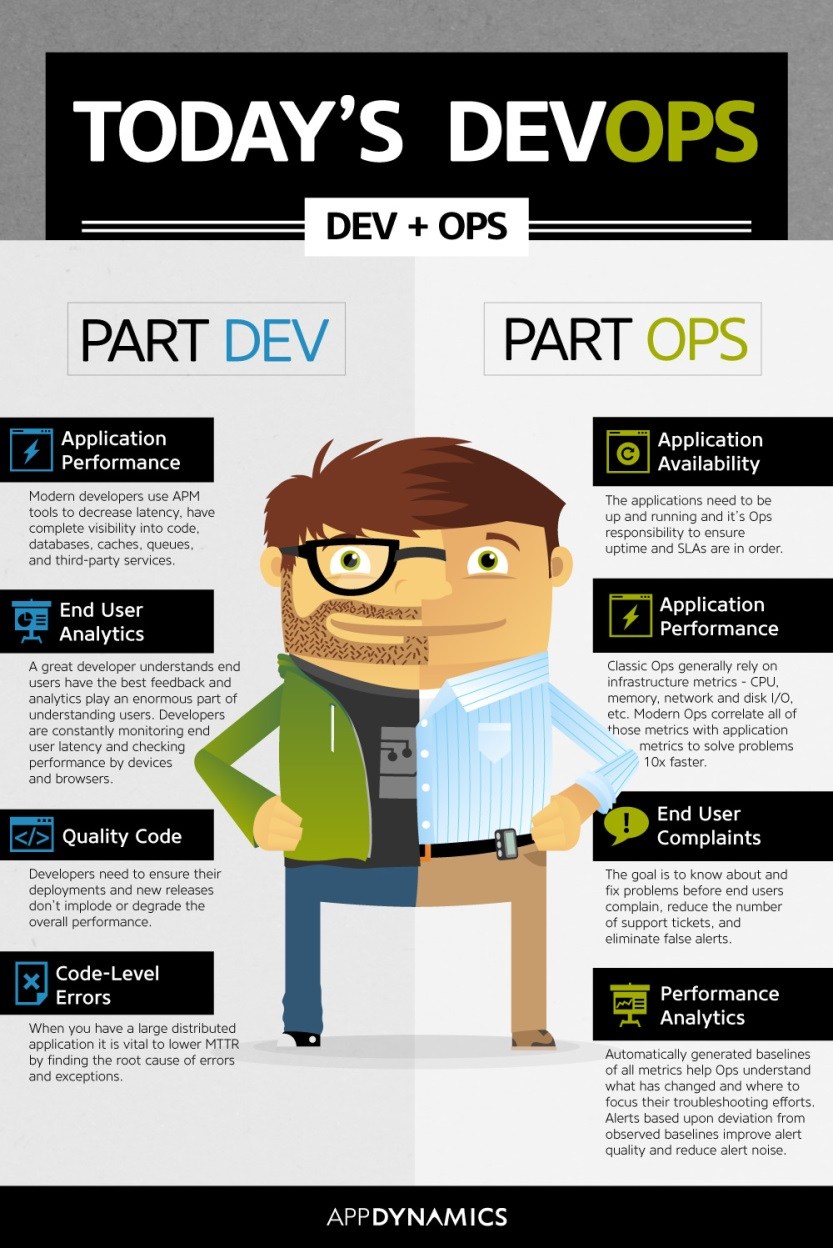
\includegraphics[scale=1.5]{images/devops.png}
  \end{center}
  \caption{DEV + OPS}
  \label{Devops}
\end{figure}

Les attentes et perspectives autour de Devops sont nombreuses :\\

\begin{itemize}
  \item \textbf{Des cycles de déploiement plus courts} : les DevOps jouent un rôle clé dans la réduction du temps du cycle de déploiement des logiciels, passant de quelques semaines à seulement quelques heures, permettant une plus grande flexibilité quant aux nouvelles fonctionnalités et changements à apporter au produit initial.
  \item \textbf{Mise à disposition de nouveaux services plus rapidement} : des déploiements fréquents associés à des délais de livraison plus rapides permettent une agilité opérationnelle.
  \item \textbf{Une satisfaction client améliorée} : grâce à des applications ciblées et de qualité, conformes aux retours clients end to end.
  \item \textbf{Des coûts réduits} : L’automatisation permet aux équipes de réaffecter des ressources précieuses à des tâches à plus haute valeur.
  \item \textbf{Conformité et Gouvernance} : Automatisation du tracking et reporting end-to-end sur les phases de livraison/déploiement contenu.\\
\end{itemize}

\section{« The Wall of Confusion »}

\section{La Culture}

\section{« Infrastructure As Code »}

http://blog.octo.com/et-si-devops-nous-emmenait-vers-tdi-test-driven-infrastructure/


  \chapter{Intégration Continue} \label{ContinousIntegration}

  \section{Histoire}
  Dans l’industrie logicielle, l’intégration d’un projet est souvent un moment lourd et douloureux. La mise en commun des différents modules composant l’application entraine généralement de graves problèmes d’intégration. Les modules fonctionnent correctement individuellement mais se confrontent à des problèmes de synergie. La résolution de ces problèmes demande un effort important qui s’accroissent avec la complexité du système. L’introduction des techniques et méthodologies de l’Intégration Continue, estompe les problèmes d’intégration jusqu’à les réduire en un non-évènement.\\

  \begin{quotation}
    \emph{« Continuous integration is the practice of making small well-defined changes to a project’s code base and getting immediate feedback to see whether the test suites still pass. »}
  \end{quotation}

  \begin{quotation}
    \emph{« L'intégration continue est la pratique de faire de petits changements bien définis à la base du code source d'un projet et d'obtenir une rétroaction immédiate pour voir si les suites de test passent toujours. »} Paul Duvall \cite{Duv07}.\\
  \end{quotation}

  L’idée d'Intégration Continue a été développée par la communauté Extreme Programming (XP) et décrite par Kent Beck dans son livre « Extreme programming explained » \cite{Bec99}. Elle s'articule autour de douze pratiques de développement agile. Son but étant de prévenir les problèmes décrits ci-dessus désignés comme « integration hell » (l’enfer de l’intégration) par Ron Jeffries en 2001. Martin Fowler a également été l'un des premiers contributeurs ayant écrit sur l’Intégration Continue \cite{Fow00}. Plus tard, ces travaux ont été poursuivi par Paul Duvall qui a écrit tout un livre à propos de l’intégration \cite{Duv07}.

  Martin Fowler \cite{Fow00} désigne 10 principes clés pour réussir une Intégration Continue efficace :\\

  \begin{itemize}
    \item maintenir un référentiel de source unique,
    \item automatiser la construction de l’application (build),
    \item automatiser les tests,
    \item valider quotidiennement les modifications au niveau de la branche principale du contrôle de version (commit),
    \item créer une build d’intégration à chaque commit sur la branche principale,
    \item assurer une build rapide,
    \item effectuer les tests dans un environnement clone de la production,
    \item assurer la disponibilité pour tous des derniers livrables,
    \item assurer une visibilité pour tous,
    \item automatiser le déploiement.\\
  \end{itemize}

  \section{L'Intégration Continue comme un processus}
  L’Intégration Continue est un processus où le logiciel est construit - buildé - à chaque changement. Cela signifie que lorsqu’une modification apportée par un développeur est détectée dans le code source, une construction - build - automatique est déclenchée sur une machine de build séparée. La build contient plusieurs étapes prédéfinies comme la compilation, les tests, la génération de métrique du code source et le déploiement - entre autres. Une fois cette construction terminée, un rapport est envoyé aux membres du projet spécifié. Le rapport de compilation indique le résultat de chaque étape de la build avec des informations détaillées sur les erreurs qui ont pu y survenir.\\\\

  Martin Fowler \cite{Fow00} décrit l’Intégration Continue comme :\\
  \begin{quotation}
    \emph{« Continuous Integration is a software development practice where members of a team integrate their work frequently, usually each person integrates at least daily - leading to multiple integrations per day. Each integration is verified by an automated build (including test) to detect integration errors as quickly as possible. Many teams find that this approach leads to significantly reduced integration problems and allows a team to develop cohesive software more rapidly. »}
  \end{quotation}

  \begin{quotation}
    \emph{« L'Intégration Continue est une pratique de développement logiciel où les membres d'une équipe intègrent leur travail régulièrement, chaque développeur intègre au moins quotidiennement une version - conduisant à de multiples intégrations journalières. Chaque intégration est vérifiée par une build automatique (y compris le test) pour détecter les erreurs d'intégration le plus rapidement possible. De nombreuses équipes trouvent que cette approche conduit à réduire considérablement les problèmes d'intégration et permet à l'équipe de développer des logiciels cohésifs plus rapidement. »}\\
  \end{quotation}

    \subsection{Les bénéfices de l’Intégration Continue}\label{Benefits}
    Selon Paul Duvall \cite{Duv07}, l'intégration logicielle n’est pas un problème dans les petites équipes (un à deux développeurs), mais lorque le nombre de collaborateurs se multiplie ou que diverses équipes commencent à travailler ensemble sur un même projet, l'intégration logicielle devient un problème, car plusieurs acteurs peuvent être amenés à modifier simultanément des morceaux de code devant fonctionner ensemble. Vérifier que les divers composants logiciels interdépendants continuent de fonctionner correctement ensemble soulève la nécessité d'intégrer plus tôt et plus souvent. Les points suivants décrivent les différents effets bénéfiques que Paul Duvall a été en mesure d'identifier.

      \subsubsection{Réduire les risques}
      En intégrant plusieurs fois par jour, les risques de dysfonctionnement sont considérablement réduits. Les problèmes sont remontés dès leur intégration et peuvent même être la cause d’un rejet d’intégration. Ceci étant possible par l’intégration, l’exécution de tests et l’inspection automatiquement du code source après chaque modification.

      \subsubsection{Générer des logiciels déployables}
      L'un des objectifs du développement logiciel agile est de déployer tôt et souvent. L’Intégration Continue aide à atteindre cet objectif en automatisant les étapes de production des logiciels déployables. Des logiciels déployables et fonctionnels est l'avantage le plus évident de l’Intégration Continue du point de vue extérieur, car le client ou l'utilisateur final est généralement peu intéressé par le fait que l’Intégration Continue ait été utilisé dans le cadre de l'assurance qualité. Il est aussi l'atout le plus tangible, étant le résultat final de l’Intégration Continue.

      \subsubsection{Permettre une meilleure visibilité du projet}
      Le fait que le processus d’Intégration Continue s’exécute régulièrement fournit la capacité à remarquer les tendances et à prendre des décisions sur la base d’informations réelles. Sans Intégration Continue, les informations doivent être recueillies manuellement, requérant du temps et des efforts. Le processus d’Intégration Continue fournit en temps réel les informations sur l'état de la build ainsi que de la qualité des dernières mesures tels que la couverture de test ou le nombre de violations des normes de codage définies par la convention.

      \subsubsection{Une plus grande confiance du produit}
      En ayant une Intégration Continue en place, l'équipe projet se protège contre certaines actions négatives portées aux codes sources. L’Intégration Continue agit comme un filet de sécurité, il repère les erreurs tôt et régulièrement. Ce qui se traduit par une plus grande confiance en l'équipe. Même des changements importants peuvent être faits avec confiance.

    \subsection{Le cycle de travail de l’Intégration Continue}
    Alors que l’Intégration Continue est généralement orchestrée par un serveur d’Intégration Continue, c’est aussi une façon de travailler. L'idée principale est d'intégrer les changements au code source aussi souvent qu’il y ait du nouveau code ajoutant de la valeur à l’application, à savoir plusieurs fois par jour. Cela rend l'intégration du code plus facile du fait qu'il y a moins de code à intégrer à chaque intégration. Il contribue également dans une situation où plusieurs personnes modifient la même base de code, car les développeurs auront ainsi les modifications apportées par les autres.
    L'intégration des changements au code source de base comporte plusieurs étapes. Le cycle de travail est illustré dans le schéma suivant (Voir Figure \ref{IC workflow}). Il est basé sur les idées présentées par Martin Fowler \cite{Fow00} avec une phase de mise à jour supplémentaire, après l'exécution des tests. Cette phase de mise à jour est nécessaire dans la situation où le test prend du temps, de sorte qu'il pourrait déjà y avoir de nouvelles modifications intégrées pendant notre phase de test.\\

    \begin{enumerate}
      \item récupérer le code source du référentiel (Check-out),
      \item modifier le code et créer les tests pour les modifications,
      \item vérifier si quelqu'un d'autre a modifié le code source,
      \item exécuter tous les tests afin de vérifier que les modifications n’aient pas altéré le bon fonctionnement de l’application,
      \item vérifier à nouveau que le code source n'ait pas changé,
      \item valider les modifications dans le référentiel (Check-in),
      \item démarrer un nouveau cycle.\\
    \end{enumerate}

    \begin{figure}
      \begin{center}
        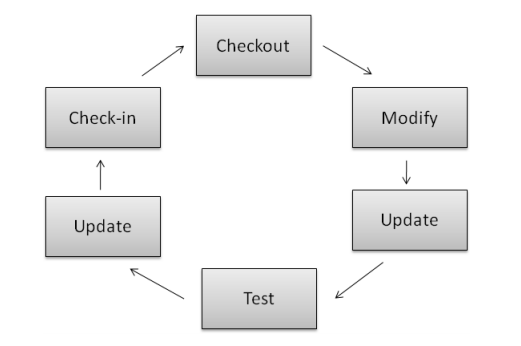
\includegraphics[scale=0.5]{images/ICWorkflow.png}
      \end{center}
      \caption{Cycle de travail de l’Intégration Continue}
      \label{IC workflow}
    \end{figure}

    Le cycle de travail commence par créer une copie du code source (hébergé sur le serveur de gestion de code) qui est sur le point d'être modifié. Si le code a été précédemment récupéré, une mise à jour est faite à la place. Le développeur effectue les changements appropriés à sa tâche (nouvelle fonctionnalité, réfactorisation du code…) et implémente les tests appropriés afin de vérifier la conformité de son développement. Un test de développement vérifie que la sortie d’une méthode, en fonction de ses entrées, soit en adéquation avec le résultat attendu.\\

    Dans un projet logiciel, il est courant que de nombreux développeurs travaillent simultanément sur une même partie de code.  Par conséquent avant d’intégrer notre partie au code source, il est nécessaire de vérifier qu’aucune modification n’ait été faite par un développeur tiers par le biais d’une nouvelle mise à jour. Dans certains cas, il est possible que d’autres développeurs aient modifié exactement les mêmes lignes de code que nous, produisant ainsi un ou plusieurs conflits. Dans ce cas, les conflits doivent être immédiatement résolus et tous les tests ré-effectués. Il est possible que dans cet intervalle une nouvelle version soit disponible sur le référentiel, l'étape précédente doit être répétée jusqu'à ce qu'aucun nouveau changement ne soit détecté. Une fois cette synchronisation effectuée le check-in peut être fait.

    \subsection{Comment l’Intégration Continue s’appuie-t-elle sur d’autres pratiques de développement}\label{Developers}
    L’Intégration Continue comprend un ensemble de règles que tous développeurs doient suivre :

    \begin{enumerate}
      \item effectuer régulièrement des commits,
      \item ne pas effectuer de commit du code buggé,
      \item régler les problèmes et builder immédiatement,
      \item écrire des tests de développement automatisés,
      \item tous les tests et métriques doivent être valides,
      \item exécuter en local ses builds,
      \item éviter de travailler avec du code buggé.\\
    \end{enumerate}

    Ces règles ne sont pas nouvelles dans le monde du développement logiciel et sont aussi adoptées par d'autres pratiques de développement. Par conséquent, si des pratiques telles que les tests de développement, les normes de codage, le refactorisation et la propriété collective sont déjà mises en place au sein du projet, il est facile de commencer à utiliser l’Intégration Continue. Ces pratiques doivent être rigoureusement appliquées au travers de l’Intégration Continue sous peine d’empêcher les autres collaborateurs du projet de correctement travailler. Prenons par exemple le cas d’un développeur ayant remanié une partie du code source et cassé quelques tests. Ne l’ayant pas remarqué, faute de n’avoir pas exécuté les tests, il valide ses changements dans le référentiel. La build échoue du faite que la règle « tous les tests doivent être au vert » n’est pas suivie. Maintenant si un autre développeur commence à travailler avec le code du référentiel, la première chose qu'il doit faire est de fixer ce qui a été cassé par son collègue. Et cela peut prendre beaucoup de temps si cette personne ne connaît pas la partie de code qui provoque l’échec des tests.

  \section{L’Intégration Continue est un mélange de personnes et de systèmes}

    \subsection{Le développeur}
    Pratiquer l’Intégration Continue exige de la discipline de la part des développeurs. Ils devront appliquer avec rigueur les pratiques de développement vues précédemment. Une fois le développement de la tâche effectué, le développeur doit exécuter une build sur sa propre machine de développement. On appelle cela une build privée. Cette étape permet de vérifier que les modifications apportées n’ont pas endommagé l'intégration avec le reste du code source. Il est important d'exécuter la build privée avant de valider les changements dans le référentiel de contrôle de version, car soumettre un code erroné peut empêcher les autres développeurs de correctement travailler. Une fois l’exécution de la build privée effectuée avec succès, le développeur peut valider les modifications et les tests. Si l'intégration de la build échoue malgré ses précautions, réparer cette build est la priorité numéro un.

    \subsection{Le référentiel de contrôle de version}\label{SCM}
    L'intégration continue ne peut pas se faire sans référentiel de contrôle de version. Le référentiel de contrôle de version, également connu sous le nom de gestionnaire de code source (Source Control Manager), est un système utilisé pour stocker le code source et d'autres aspects du logiciel (comme la documentation, les specs, ...) de manière centralisée. Il assure également le suivi de l'historique des versions et modifications effectuées au cours du développement. Les développeurs logiciels ont la possibilité de revenir à une version antérieure ou à la révision d'un logiciel et de prendre connaissances des changements apportés sur toutes révisions données. Ce référentiel fournit un point d'accès unique au code source pour les développeurs et le système d’Intégration Continue. Il peut être constitué de différentes branches du logiciel stocké. Une branche peut être créée pour la réécriture majeure d’un morceau de code ou pour le prototypage d’une idée intéressante qui pourrait ne pas se retrouver dans le produit final. La build d’intégration est exécutée sur la branche principale du référentiel de contrôle de version \cite{Duv07}. « Master » est la branche de code source où la plupart de la mise au point a lieu. Certains systèmes de contrôle de version appellent cela « tunk » ou « head ». La ligne principale se doit d’être toujours stable et la build d’intégration ne doit jamais échouée quand elle est intégrée au référentiel.

    \begin{figure}
      \begin{center}
        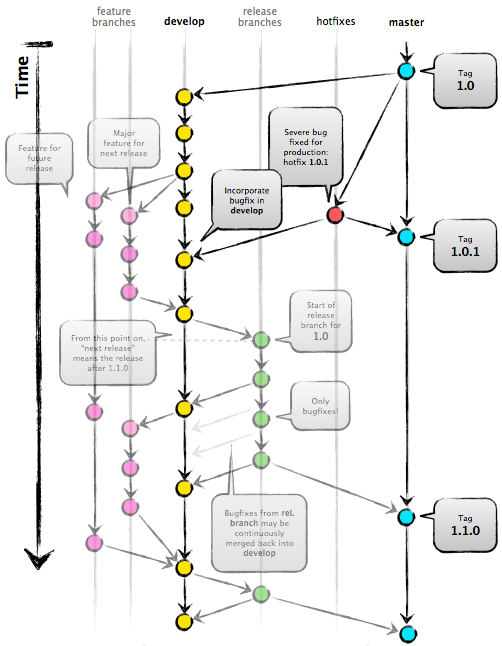
\includegraphics[scale=0.7]{images/gitFlow.png}
      \end{center}
      \caption{Ligne de temps d'un référentiel de contrôle de version}
    \end{figure}

    \subsection{Le serveur d’Intégration Continue}\label{ServeurCI}
    Le serveur d’Intégration Continue est l'orchestrateur de l'ensemble du processus. Il exécute la build d'intégration lorsqu'une modification a été apportée au référentiel. Trois approches sont à prendre en compte.\\

    La première est la configuration d’un « post commit hook » au niveau du gestionnaire de code source. Le référentiel de contrôle de version peut-alors immédiatement avertir le serveur d’Intégration Continue qu’une modification a été ajoutée et validée. De cette façon une build d’intégration est exécutée à chaque commit.\\

    Une autre approche, dénommée « polling approach » \cite{Duv07} est de vérifier les changements à intervalles réguliers (de l’ordre de la minute). De ce fait plusieurs changements peuvent être effectués entre chaque build.\\

    La troisième et dernière option, consiste à intégrer une copie du référentiel principal, accessible uniquement par le serveur d’Intégration Continue, au niveau du serveur lui-même \ref{IC server}. Les développeurs n’ont ainsi accès qu’au référentiel clone du serveur d’Intégration Continue. Ce dernier peut alors être configuré afin de rejeter les modifications apporté au référentiel ne respectant pas les tests ou les métriques qualités prédéfinies. Garantissant ainsi la qualité de l’application.\\\\

    \begin{figure}
      \begin{center}
        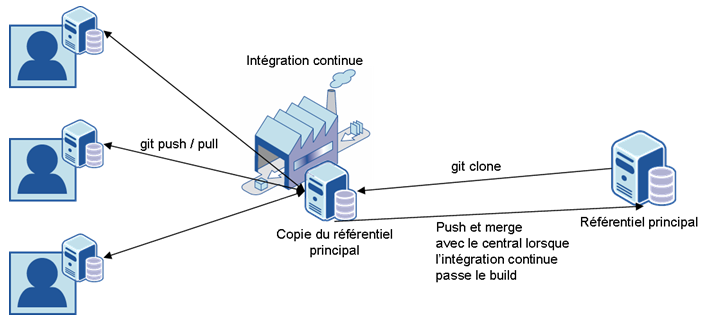
\includegraphics[scale=0.5]{images/ICServer.png}
      \end{center}
      \caption{Organisation d'un serveur d'Intégration Continue}
      \label{IC server}
    \end{figure}

    Le serveur d’Intégration Continue fournit également une vue, généralement une page web, qui expose l'état de santé de tous les « build jobs »\footnote{Build jobs : cela correspond aux différentes tâches du processus de build.} et affiche leurs résultats en temps réel (Voir Figure \ref{Jenkins build jobs}). Ce tableau de bord peut être affiché, par exemple, sur un grand écran dans la salle de l'équipe de développement pour donner un aperçu rapide et en temps réel des tâches effectuées sur le serveur et voir ainsi si des builds sont en cours d'exécution. De nombreux serveurs d’Intégration Continue proposent également un type de visualisation basé sur les principes des feux de circulation ou de météo afin de connaitre l’état des builds d’Intégration.\\

    Toutes les fonctionnalités d’un serveur d’Intégration Continue ne sont pas nécessaires pour faire de l’Intégration Continue. De nombreux scripts personnalisés peuvent effectuer les mêmes tâches, mais avoir un serveur conçu à cet effet aide beaucoup \cite{Duv07}. De plus en plus de solutions propriétaires ou open source\footnote{Open source : logiciel libre redistribution, d'accès au code source et de création de travaux dérivés.} performent le marché en offrant un environnement d’Intégration Continue stable et complet.\\

    Dans sa forme la plus simple, l’Intégration Continue pourrait être mise en place avec un seul ordinateur dédié (serveur) exécutant des scripts afin de vérifier le code source du référentiel, lancer une build d’intégration et envoyer des rapports une fois la build terminée. Le serveur d’Intégration Continue offre une autre possibilité en fournissant une interface utilisateur afin de configurer les multiples « build jobs ».

    \begin{figure}
      \begin{center}
        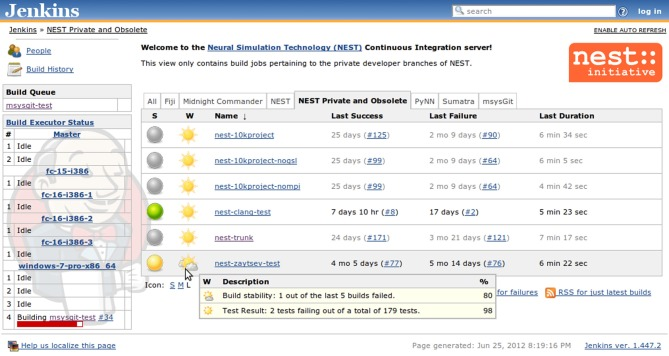
\includegraphics[scale=0.5]{images/jenkinsBuildJobs.png}
      \end{center}
      \caption{Tableau de bord d'un serveur d'Intégration Continue Jenkins}
      \label{Jenkins build jobs}
    \end{figure}

    \subsection{Les scripts de construction (build)}
    Généralement, la plupart des étapes d’une build sont définies en utilisant un script de compilation. Un script de compilation peut être constitué d'un ou plusieurs scripts et est utilisé, par exemple, pour compiler, tester, contrôler et déployer des logiciels. Toutes les actions pouvant être automatisées pour construire et déployer des logiciels doivent être automatisées. Cela permet d'économiser du temps (et donc de l'argent) tout en garantissant la qualité de l'exécution. Il existe de nombreuses techniques disponibles comme Ant (Java), Make (C/C++) ou Scons (Python).\\

    Certains développeurs utilisent leur environnement de développement intégré (IDE) pour builder leurs logiciels. Dans ce cas la build ne pourra être encadrée par l’Intégration Continue. L’intégration Continue nécessite que celle-ci puisse être exécutée indépendamment de tout IDE \cite{Duv07}.

    \subsection{Les mécanismes de feedback}
    Lorsque la build d'intégration est terminée, les résultats doivent être accessibles dès que possible. La capacité à fournir un feedback rapide est l'un des avantages de l’Intégration Continue. La rétroaction est disponible immédiatement une fois la build terminée. Elle peut être diffusée par différents canaux; tableau de bord, courrier électronique, flux RSS. En cas de build défectueuse, la réparation peut démarrer immédiatement après réception de l'avis.\\

    Certains pionniers commencent même à intégrer le terme de « monitoring continue » dans l’ingénierie logicielle en complément de l’Intégration Continue. Le monitoring continu consiste à avoir un affichage visible par tous les membres de l’équipe de développement, actualisé en temps réel, donnant un feedback direct sur l’état des différentes builds simplifié et directement interprétable. Cet affichage est dans la plupart du temps un moniteur, mais d’autres solutions plus amusantes, telles que la lampe à lave ou une « ambient orb » commencent à s’imposer \cite{Swa04}.

    \subsection{Les machines de build d’intégration}
    Un serveur d’Intégration Continue à besoin d'un hôte pour fonctionner. La machine de build d’intégration (ou nœud) est une machine distincte qui doit imiter l'environnement de production. Si possible, elle doit fonctionner avec le même système d'exploitation, la même version de serveur de base de données et les mêmes versions de librairies doivent être utilisées, comme il est prévu en production. Chaque différence augmente le risque des tests de ne pas détecter les problèmes liés à l’environnement \cite{Fow06}.\\

    Dans le cas où de nombreux « build jobs » sont configurés pour l’application, pour réduire la durée de la build et ainsi augmenter la rapidité de la rétroaction il peut être nécessaire de paralléliser les tâches sur plusieurs machines (scalabilité horizontale). Certains logiciels de serveur d’Intégration Continue fournissent une architecture maître-esclave qui permet ainsi de diviser la charge de travail sur plusieurs hôtes.\\

    Parfois plusieurs environnements sont nécessaires pour builder sur différentes plates-formes. La virtualisation des serveurs apportent la réponse à ce problème. En utilisant une infrastructure de virtualisation bien établie, il est assez facile d’exécuter des instances esclaves multiples sur un seul nœud physique. Ces instances pouvant fonctionner sous différents systèmes d’exploitation. Certains logiciels de serveur d’Intégration Continue offre la possibilité à la build d’intégration de fonctionner simultanément sur ces différentes instances et de collecter les résultats pour chaque environnement.\\

  \section{Caractéristique de l’Intégration Continue}\label{Features of Continuous Integration}
    \subsection{Inspection Continue}
    Le code source peut être examiné manuellement et/ou automatiquement. La revue de code manuelle peut être effectuée selon deux principes, le « pair programming » (écriture du code en binôme) ou le « code review » (session collective de relecture du code). Elle améliore la qualité algorithmique et syntaxique du code source de l’application et permet aux développeurs d’échanger sur les bonnes pratiques. Pour une revue de code automatique, de nombreux analyseurs de code statique sont disponibles selon les langages de développement. Ces outils analysent les fichiers sources dans le but de souligner les violations de règles prédéfinies propre au langage et d’améliorer la syntaxe de nos lignes de code.\\

    La différence entre la revue de code manuelle - faite par des humains - et la revue de code automatique - faite par des outils d’analyses - est double. Exécuter les analyseurs de code statique est peu cher, et une fois automatisés, ils garantissent une relative propreté au code source. De plus un ordinateur est toujours objectif et ne se lasse pas d’inspecter l’intégralité du code à chaque fois qu’un changement est engagé dans le référentiel de contrôle de version.\\

    Les analyses statiques de code automatisé sont efficientes pour des grandes bases de code. Elles permettent aux développeurs de se concentrer sur les parties importantes. Elles offrent des métriques de qualité sous la forme de rapport d’inspection après chaque exécution. Les revues automatisées ne remplacent pas les revues manuelles, elles permettent de recentrer l’intelligence humaine là où elle est nécessaire.\\

    De nombreux IDE (environnement de développement intégré) proposent des fonctionnalités d’inspection pour aider les développeurs dès l’écriture du code avec une mise en forme automatisée, la mise en évidence des variables non utilisées, l’utilisation illégale de certain élément… Il est fortement encouragé de les utiliser mais ne remplace en aucun cas les revues de code.\\

    Il existe également des outils qui proposent de réécrire certains bouts de code selon une convention particulière, de détecter les blocs de code en double…

      \subsubsection{Rapport d’inspection}
      Les outils d’analyse statique de code fournissent un grand nombre de mesures et de rapports, encore faut-il les interpréter. Depuis quelques décennies des chercheurs étudient ces mesures afin de trouver une corrélation entre les défauts soulignés par les analyses et le code source.\\

      Une des principales mesures étudiées est la complexité cyclomatique, qui quantifie la complexité du code source en comptant le nombre de chemins distincts au travers d'un programme représenté sous la forme d'un graphe \cite{Kan03}. Les analystes suggèrent une complexité de 10 car plus grand est ce nombre, plus important sera le risque de défauts \cite{Wat96}. Le moyen le plus efficace pour réduire la complexité cyclomatique d’une application est d'appliquer la technique de la méthode d'extraction et de distribuer la complexité en petites méthodes, plus faciles à gérer, et donc plus testables \cite{Duv07}.\\

      Outre les problèmes de complexités, les rapports d’inspection nous fournissent des mesures sur les problèmes liés à l’architecture de notre application; « l’afferent coupling » et « l’efferent coupling ». Ces métriques comptent les nombres de dépendances vers, où à partir d’un objet, soulignant ainsi les risques de responsabilités ou de dépendances trop fortes. Elles permettent de déterminer le niveau de risque dans le maintien et l’évolutivité du code. Duvall introduit l'utilisation de ces deux valeurs combinées pour calculer une valeur d'instabilité.\\

      \begin{center}
          $Instability=\frac{EfferentCoupling}{EfferentCoupling + AfferentCoupling}$\\
      \end{center}

      La compréhension de ces mesures et de l'analyse des rapports d'inspection peut une réelle plus-value sur le temps investi. Les problèmes de maintenabilité peuvent être repérés dès le début et les risques de défauts peuvent être réduits.

    \subsection{Compilation du code source}
    La compilation du code source est l'une des caractéristiques de base du système d’Intégration Continue. La compilation crée des exécutables binaires à partir de sources lisibles (pour les développeurs). Lors de l'utilisation des langages dynamiques comme Python ou Ruby la compilation est différente. Les binaires ne sont pas compilés, à la place les développeurs ont la possibilité d'effectuer un checking strict, qui peut être considéré comme de la compilation dans le contexte de ces langues \cite{Duv07}.

    \subsection{Tests}
    Les tests sont la partie la plus vitale de l’Intégration Continue. Beaucoup considèrent qu’une Intégration Continue sans automatisation du contrôle continu ne peut être un Contrôle Continue \cite{Duv07}. Il est difficile d'avoir confiance dans les changements du code source sans une bonne couverture de test. Les tests peuvent être automatisés en utilisant des outils de tests unitaires tels que JUnit (Java), NUnit (C\#), ou d'autres framework\footnote{Framework : ensemble d'outils et de composants logiciels.} de xUnit. Certains de ces frameworks peuvent également générer des rapports machines lisibles, qui peuvent être analysés et utilisés pour générer des représentations graphiques telles que des pages Web ou des tableaux (Voir Figure \ref{xUnit output}).

    \begin{figure}
      \begin{center}
        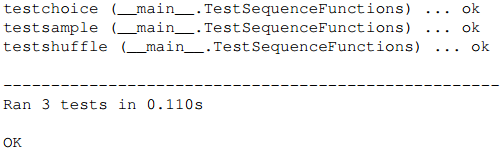
\includegraphics[scale=0.8]{images/tests.png}
      \end{center}
      \caption{xUnit output}
      \label{xUnit output}
    \end{figure}

      \subsubsection{Niveaux de tests}
      Le test peut être effectué à différents niveaux \ref{Testing levels}. Le plus bas niveau de test est appelé test unitaire. Une unité est la plus petite partie d’une application testable. Cela correspond à une fonction ou une méthode dans une classe. Le but des tests unitaires est de vérifier que les différentes parties du code fonctionnent comme elles le devraient. Ils assurent la stabilité du code en testant chaque unité unitairement. Les régressions sont ainsi remontées très rapidement ce qui permet de manipuler le code source avec confiance. Les tests unitaires sont généralement écrits par le développeur qui a également écrit le code. Une bonne pratique des tests unitaires est de commencer par écrire les tests et d’ensuite les valider par le code. C’est ce qu’on appelle le « Tests Driven Development » (TDD) ou Développement Dirigé par les Tests ».\\

      Le niveau suivant est le test d'intégration. Dans ce contexte d’Intégration nous devons vérifier que les modules individuels du logiciel fonctionnent aussi en tant que groupe.\\

      \begin{quotation}
        \emph{« Le test d'intégration identifie les problèmes qui se produisent lors de la combinaison d'unités. En utilisant un plan de test exigeant que vous testiez chaque unité et que vous vérifiez la viabilité de chacune d'elles avant de les combiner, vous savez que les erreurs découvertes lors de la combinaison d'unités concernent probablement l'interface entre les unités. Cette méthode réduit le nombre de possibilités à un niveau beaucoup plus simple d'analyse. »} Microsoft \cite{Mic16}.\\
      \end{quotation}

      Le troisième niveau teste les API d’un point de vue externe, sans se préoccuper de fonctionnement interne du système. Le test système analyse le flux de retour de l’API en fonction de son flux d’entrée afin de détecter les défauts à la fois dans les inter-assemblages mais également au sein du système dans son ensemble. Cette méthode est appelé « boîte noire ».\\

       Le test fonctionnel est le quatrième niveau de test majeur. Il assure la stabilité de l’application en reproduisant le parcours d’un utilisateur sur le navigateur. Il teste le bon fonctionnement de l’application et remontent les régressions fonctionnelles.\\

       D’autres niveaux de test existent, tel que le test applicatif qui assure la sécurité et la compatibilité, le test d’IHM qui fiabilise l’ergonomie et la visibilité, le test de charge qui veille à la performance et à la robustesse de l’application...

       \begin{figure}
         \begin{center}
           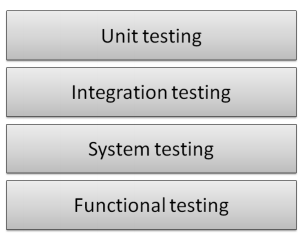
\includegraphics[scale=0.7]{images/testingLevels.png}
         \end{center}
         \caption{Les principaux niveaux de test}
         \label{Testing levels}
       \end{figure}

      \subsubsection{Exécuter les tests plus rapides en premier}
      Lorsque le logiciel se développe, le nombre de tests augmente, ce qui se traduit par une hausse du temps d’exécution des tests lors de la build d’intégration. Si l’ensemble des tests est exécuté en une seule fois cela peut prendre du temps et ainsi faire perdre le bénéfice de la rétroaction rapide. Pour faire face à ce syndrome, les tests doivent être classés du plus rapide au plus lent en terme d’exécution. Les tests peuvent aussi être divisés en plusieurs étapes. Les rapports seront envoyés à la fin de chaque étape garantissant un feedback rapide.\\

      Les tests unitaires nécessitent peu de temps lors de leur mise en place et sont les tests les plus rapides à exécuter. L’exécution d’un test unitaire ne doit pas excéder la fraction de seconde. Ces tests sont exécutés de nombreuses fois par jour par les développeurs. La rapidité d’exécution est primordiale sinon les tests deviennent une méthodologie de développement à éviter ce qui est contraire au principe de l’Intégration Continue \cite{Duv07}. Les tests unitaires sont donc de bons candidats pour être exécuter au cours de la première étape.\\

      La configuration des tests d'intégration et des tests système nécessitent beaucoup plus de temps que celle des tests unitaires. La mise en place de la (des) base(s) de données avec des données de test et de lancement réel de l’application sont des tâches relativement chronophages. L’exécution de ces tests peut être une étape longue. Les tests d’intégration et système peuvent être exécutées dans des étapes ultérieures ou à des intervalles périodiques. Par exemple nous pouvons exécuter une suite complète de tests de plusieurs heures tous les soirs. Nous appelons ce processus Daily Build \cite{McC96}.

      \subsubsection{Ecrire des tests d’échecs}
      L’écriture et l’exécution automatique des tests avec l’Intégration Continue diminue la fréquence des logiciels défectueux. Mais l’Intégration Continue n’est pas infaillible \cite{Duv07}. Si un défaut est trouvé, il doit être immédiatement fixé et pour éviter qu'il se reproduise, un test défectueux devra être implémenté. L'idée sous-jacente est d’améliorer continuellement la qualité de l’application.

      \subsubsection{Différences entre inspection et test}
      Le test (vu précédemment) est dynamique et exécute l’application, ou un fragment de l’application, pour tester ses fonctionnalités. L’inspection, quant à elle, analyse le code selon un ensemble de règles prédéfinies. Les deux sont des concepts similaires dans le sens ou aucun ne modifient le code source, ils ne font que remonter les problèmes résidant dans l’application.

    \subsection{Base de données d’intégration}
    L’Intégration Continue ne se limite pas à la construction du code source, elle peut également être utilisée dans le développement des bases de données. Les bases de données sont des parties intégrantes des applications et ont donc besoin d’être intégrées dans le processus d’Intégration Continue. La création d’une base de données fonctionnelle lors d’une build d’intégration nécessite un ensemble de scripts stocké dans le référentiel de contrôle de version. Ces scripts comprennent les définitions des tables, les procédures stockées, le partitionnement... L’exécution des tests fonctionnels nécessite des données « réelles » afin de garantir un environnement proche de la production. Des scripts de « données », exécutés après la création de la base de données complètent la mise en place d’une base de données fonctionnelle.\\

    Par exemple, lorsqu’un développeur ou un administrateur de base de données (DBA) apporte une modification à script de base de données et le valide au niveau du système de contrôle de version (check-in), la build d’intégration (la même que celle utilisée pour l’intégration du code source) construit la nouvelle base de données et lance les tests.

      \subsubsection{Test unitaire sur les fonctions de base de données}
      Pour des raisons de sécurités et de performances les fonctions propres aux bases de données sont stockées et exécutées par elles-mêmes. On les appelle alors « procédures stockées ». Comme pour les méthodes de l’application ces procédures doivent être testées et automatisées par des scripts qui seront exécutés lors de la build d’intégration.

    \subsection{La documentation}
    Les méthodes de développement agile mise en place par eXtreme Programming mettent l'accent sur le « working software over comprehensive documentation » \cite{HF01}. La documentation est directement intégrée dans le code source et respecte les conventions de nommage propre à chaque langage. Lorsque ce dernière est correctement intégrée dans le code source l'Intégration Continue peut utiliser des outils afin de mettre à jour la documentation à chaque construction (Javadoc, NDoc, Pydoc, ...). Ces outils peuvent également être utilisés pour créer des diagrammes de classes ou de dépendances. Tous ces documents générés automatiquement sont basés sur le code source présent dans le référentiel de contrôle de version ce qui offre la documentation et le status d'avancement en temps réel de l'application.

  \section{Déploiement Continu}
  L'un des objectifs de l’Intégration Continue est d'avoir un logiciel prêt et fonctionnel pour le déploiement à tout moment du développement. Toutes les étapes vues précédemment sont des parties du processus de déploiement visant à générer les artefacts de logiciels fournis avec les dernières modifications de code disponibles dans un environnement de test \cite{Duv07}. Une fois l’application packagée il est possible de l'installer automatiquement sur les serveurs de production avec le Déploiement Continu. Celui-ci constitue l'ensemble des outils, méthodologies et bonnes pratiques permettant le déploiement de l'application sur un environnement de production en un clic et sans intervention humaine (sinon nous parlons de Delivery Continu et non de Déploiement Continu).

    \subsection{Les bonnes pratiques du Déploiement Continu}
    Pour cela Paul Duvall définit six bonnes pratiques de haut niveau afin de réaliser convenablement un bon Déploiement Continu:\\
    \begin{itemize}
      \item labeliser les actifs d'un référentiel,
      \item produire un environnement propre, exempt d'hypothèses,
      \item générer et étiqueter une version directement à partir du référentiel et l'installer sur la machine cible,
      \item effectuer les tests avec succès à tous les niveaux dans un clone de l'environnement de production,
      \item créer des rapports de rétroaction de build,
      \item	si nécessaire, la release peut être annulée en utilisant des étiquettes dans le système de contrôle de version.\\
    \end{itemize}

      \subsubsection{Etiqueter (labéliser) les actifs d’un référentiel}
      La création de label au niveau du référentiel facilite l'identification et le suivi des actifs, en définissant clairement un groupe de fichiers comme appartenant à un ensemble. De plus, les étiquettes permettent un suivi historique d'un groupe de fichiers et pas seulement comme des fichiers individuels qui peuvent être sur différentes versions à un moment donné \ref{Labels Referential}.

      \begin{figure}
        \begin{center}
          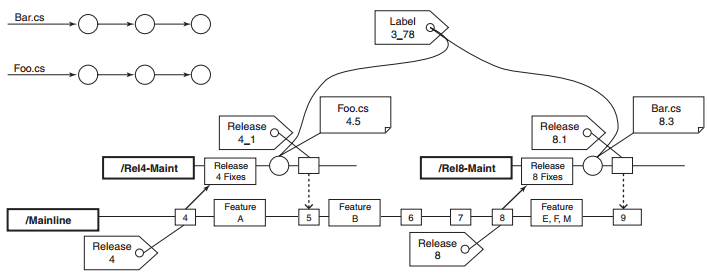
\includegraphics[scale=0.7]{images/Labels.png}
        \end{center}
        \caption{Exemple de référentiel labélisé contenant Foo.cs et Bar.cs}
        \label{Labels Referential}
      \end{figure}

      \subsubsection{Produire un environnement propre}
      Afin de réduire les risques comportementaux de l’application il est important de ne pas faire d’hypothèse sur son fonctionnement au travers des différents environnements. Idéalement l’intégralité des environnements doivent être virtualisé et automatisé afin d’être redéployé à chaque déploiement et ainsi garantir un environnement « propre ».\\
      Voici les grandes étapes de la virtualisation et l’automatisation d’un environnement :\\
      \begin{itemize}
        \item mise en place du système d’exploitation (OS),
        \item configuration de l’OS (utilisateurs, firewalls, …),
        \item mise en place des composants du serveur (serveur web, base de données, …),
        \item configuration du serveur,
        \item installation des outils tiers (frameworks web, librairies, …),
        \item	configuration des divers softwares.\\
      \end{itemize}

      \subsubsection{Etiqueter chaque build}
      Afin de créer un identifiant unique pour chaque build il est impératif que le code du référentiel ait été labélisé (cf. Etiqueter (labéliser) les actifs d’un référentiel). Le deuxième point clé est la mise en place d’un schéma de nommage commun aux diverses builds. Labéliser chaque build fournit un moyen simple de suivre efficacement la version du code et son environnement d’exécution. En outre, les défauts, les améliorations et les nouvelles fonctionnalités peuvent être émises contre cette instance de code source.\\\\

      \begin {boxedminipage} {11cm}
        Notez la différence entre une étiquette de référentiel et une étiquette de build. Les étiquettes de référentiel désignent un ensemble de fichiers non compilés tandis que les étiquettes de build désignent les fichiers binaires en sortie d’une build. Les schémas de nommage sont cependant liés. Par exemple si l’étiquette du référentiel est 4-32 celle de la build sera 4-32.01.
      \end {boxedminipage}\\

      \subsubsection{Exécuter tous les tests}
      Avant le packaging et le déploiement d’une build, l’intégralité des tests doivent être exécutés et validés, des tests unitaires aux tests fonctionnels. Ceux-ci doivent être exécutés dans un environnement aussi proche que possible que de l’environnement de production.

      \subsubsection{Créer des rapports de build}
      Les rapports de build fournissent des informations à propos des actions effectuées au cours de la build (tests, analyses statiques …), des fichiers modifiés, des issues impactées ainsi que des changements majeurs par rapport à la build précédente. Ces rapports sont généralement composés de :\\
      \begin{itemize}
        \item un rapport de test qui indique le nombre de tests effectués, le nombre de succès et d’échec et le pourcentage de code couvert par les tests,
        \item un fichier différentiel qui informe des changements exacts dans le code source,
        \item un rapport d’analyse statique qui avertit des violations des bonnes pratiques de développement,
        \item un Changelog qui recueille les notes du développeur (résolution de problèmes, nouvelles fonctionnalités ...).\\
      \end{itemize}

      \subsubsection{Capacité à effectuer un rollback}
      Quelques fois l’inévitable se produit et le logiciel déployé en production ne fonctionne plus correctement. La capacité à annuler une mise en production est inestimable dans le Déploiement Continu. Lorsque le principe d’étiquetage est correctement utilisé la demande d’une version antérieur de l’application est simple (rollback). Par ailleurs si l’ensemble de la chaine de déploiement est automatisé le temps nécessaire au rollback est minime.

    \subsection{Le pipeline de déploiement}\label{DeployementPipeline}
    L'un des défis de l'automatisation de la build et des tests est la rapidité d'exécution, de sorte que l'on puisse obtenir une rétroaction rapide. Cependant l'exécution complète de certaine tâche peut s'avérer longue. Le pipeline de déploiement \cite{Fow13} est un moyen de régler ce problème en divisant votre build en plusieurs étapes. Comme pour les tests, les étapes fournissant une rétrocation rapide seront exécutées au début du pipeline tandis que les étapes longues seront réservées pour la fin.\\

    Habituellement la prémière étape d'un pipeline de déploiement est la compilation des sources afin de fournir les binaires de l'application aux étapes suivants. Ces étapes peuvent être parallélisées sur de nombreuses autres machines. Comme son nom l'indique, la dernière étape d'un pipeline de déploiement est le déploiement de l'application dans son environnement de production.\\

    Globalement l'objectif d'un pipeline de déploiement est de détecter les changements qui conduiront à des problèmes en production. Ceux-ci peuvent inclure les performances, la sécurité ou des problèmes liés à l'utilisation. La pipeline de déploiement doit permettre la collaboration entre les différentes entités impliquées dans le projet et fournir une visibilité claire et unique sur le flux des changements du système.

    \subsection{La conteneurisation}\label{Containers}
    Le site officiel de Docker, leader mondial dans les solutions de contenerisation définit son outils comme tel:\\

    \begin{quotation}
      \emph{« Docker est un outil qui peut empaqueter une application et ses dépendances dans un conteneur virtuel, qui pourra être exécuté sur n’importe quel serveur Linux »}\\
    \end{quotation}

    Le mot clé de cette définition est conteneur virtuel. Qu’est ce qu’un conteneur virtuel?

      \subsubsection{Le conteneur virtuel}
      Le conteneur n’est pas une notion propre à Docker. Linux, par exemple, a un système de conteneur qui s’appelle LXC (LinuX Container) qui permet de gérer cet empaquetage.\\

      Un conteneur est globalement une sorte de boite, un peu comme une machine virtuelle, qui va être complètement isolée du système d’exploitation dans laquelle nous allons pouvoir installer toutes les librairies dont a besoin notre application pour fonctionner ainsi que notre application. Le conteneur étant complètement isolé du reste nous allons pouvoir le distribuer un peu partout, indépendamment du système d’exploitation.

      \subsubsection{Les avantages}
      Actuellement nos applications ont besoin de plus en plus de technologies pour fonctionner. Prenons un cas concret avec une application PHP.\\

      Une application PHP a besoin d’une certaine version de PHP, ImageMagick (pour la conversion d’images), d’une base de données, d’un système de cache, d’un serveur web (Nginx ou Apache), d’un indexeur (Elasticsearch)… Pour au final nous retrouver avec une application nécessitant de nombreuses dépendances.\\

      Le problème est que lorsque nous travaillons avec un administrateur système ou un hébergeur tiers, le déploiement de notre application peut rapidement s’avérer fastidieux. Ces derniers devront installer sur chaque serveur de déploiement les dépendances requises pour le bon fonctionnement de notre application. En tant que développeur nous ne sommes pas forcément sensibles à toutes les problématiques liées aux serveurs ce qui créé un climat hostile entre les développeurs et les administrateurs systèmes.\\

      Le gros avantage du conteneur est que ce dernier va pouvoir être livré avec l’intégralité des dépendances liées à notre application.

      \subsubsection{Conteneur VS Machine virtuelle (VM)}
      Ce que nous venons de décrire est exactement le principe de fonctionnement d’une VM. Pour comprendre la différence entre ces deux technologies voici un petit schéma issu du site officiel de Docker (Voir Figure \ref{Virtual Machine}).\\

      \begin{figure}
        \begin{center}
          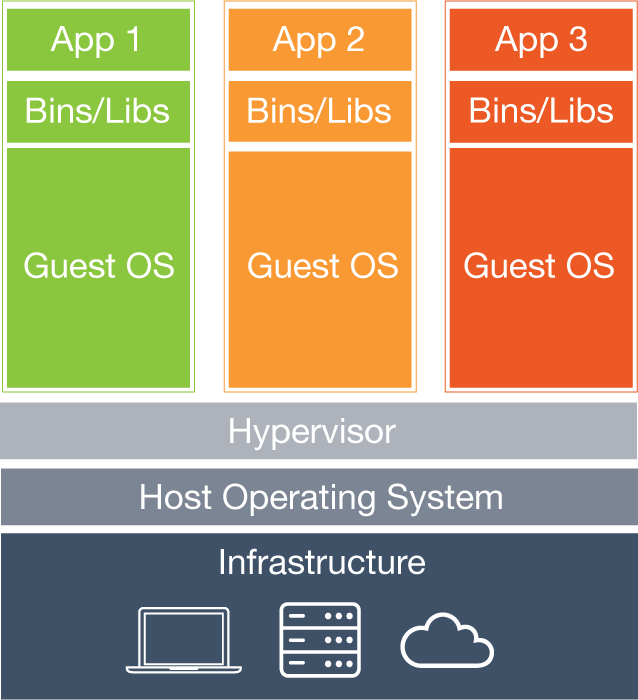
\includegraphics[scale=0.2]{images/virtualMachine.png}
        \end{center}
        \caption{Schéma de fonctionnement d'une machine virtuelle}
        \label{Virtual Machine}
      \end{figure}

      Voici la structure actuelle d’un serveur que l’on a avec des machines virtuelles. Nous nous retrouvons avec une infrastructure et par dessus un système d’exploitation qui va ensuite faire fonctionner diverses machines virtuelles. Pour schématiser nous avons un ordinateur dans un ordinateur. Le problème de cette structure est la redondance des systèmes d’exploitation. Si notre serveur héberge x machine(s) virtuelle(s), nous aurons x système(s) d’exploitation installés sur notre serveur, ce qui consomme beaucoup de ressources mémoires et processeurs.\\

      Le système de conteneur nous permet de nous absoudre de cette contrainte et de faire fonctionner nos applications directement sur le système d’exploitation du serveur hôte. Nous n'avons ainsi plus besoin de virtualiser les différents systèmes d’exploitations de nos applications, ce qui va alléger notre structure serveur (Voir Figure \ref{Container}).\\

      \begin{figure}
        \begin{center}
          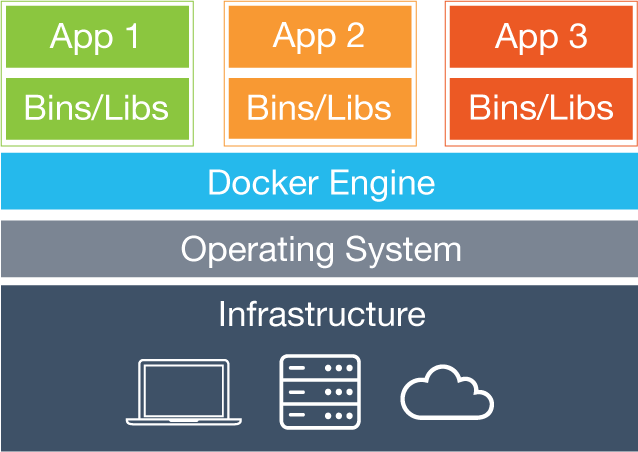
\includegraphics[scale=0.2]{images/container.png}
        \end{center}
        \caption{Schéma de fonctionnement d'un conteneur}
        \label{Container}
      \end{figure}

      \subsubsection{Les avantages}
      Les avantages de l’utilisation de conteneur sont nombreux. Nous allons nous intéresser aux quatre principaux, les gains en performance, la portabilité des conteneurs, leur scalabilité et les facilités de déploiement.\\

      Un système d’exploitation s’appuie sur de nombreux processus coûteux en mémoire et en CPU (temps de calcul d’un ordinateur). La réduction du nombre de systèmes d’exploitation à un unique OS tournant sur notre serveur hôte augmente considérablement les performances de ce dernier.\\

      Le système de boite isolée rend la technologie des conteneurs beaucoup plus portable. Si nous voulons transférer une machine virtuelle d’un serveur A à un serveur B nous devons effectuer un snapshot intégral de notre machine virtuelle et le transférer. Le problème est qu’une machine virtuelle pèse lourd. Du coup le transfert d’une VM prend beaucoup de temps.\\

      Le troisième avantage du conteneur est qu’il est plus facilement scalable. Nous allons pouvoir bouger nos petites boîtes très rapidement d’un serveur à l’autre et même les faire évoluer en terme de performance.\\

      Le dernier avantage que nous allons aborder - lié à la faculté de portage et de scalabilité de nos conteneurs - est le déploiement de ces derniers. Déployer un conteneur va être très simple. Puisqu’un conteneur est léger et qu’il embarque l’intégralité des dépendances nécessaires au bon fonctionnement de notre application nous allons pouvoir envoyer à notre administrateur système ou notre hébergeur l’intégralité de notre environnement de production.

    \subsection{La « bêta perpétuelle »}
    Le principe de la « bêta perpétuelle » a été introduit pour la première fois par Tim O’Reilly dans le manifeste du Web 2.0, qui expose le principe selon lequel:\\
    \begin{quotation}
      \emph{« Les utilisateurs doivent être considérés comme des co-développeurs, en suivant les principes Open Source (…). Avec le Web 2.0, ce principe évolue vers une position plus radicale, la bêta perpétuelle, dans laquelle le produit est développé de manière ouverte, avec de nouvelles fonctionnalités offertes sur une base mensuelle, hebdomadaire, ou même quotidienne. »}\\
    \end{quotation}

    Le terme « bêta perpétuelle » désigne le fait que notre application n’est jamais finalisée. Elle s’absout des contraintes habituelles liées au cycle de développement en « release » au profit d’une livraison en continue des nouvelles fonctionnalités.

      \subsubsection{Release early, release often}
      Derrière ce nouveau concept se cache un concept déjà bien en place chez les agilistes (du point de vue de l’itération courte) et dans le monde de l’Open Source (du point de vue de la récolte continue du feedback), le « Release Early, Release Often », traduit en français par « Publiez tôt, publiez souvent ». Cette pratique a été décrite par Eric Steven Raymond dans “La cathédrale et le bazar” où il formulait explicitement:\\
      \begin{quotation}
        \emph{« Publiez tôt. Publiez souvent. Et écoutez vos clients »}\\
      \end{quotation}

      Cette méthodologie vise à réduire les temps de développement et améliorer l’implication de l’utilisateur dans la conception du logiciel afin de créer un produit correspondant à ces attentes et ainsi éviter la création d’un logiciel que personne n’utilisera.

      \subsubsection{Les services en ligne (Software As A Service)}
      Le concept de « bêta perpétuelle » a été rendu possible grâce au Cloud Computing et plus particulièrement à la généralisation du service en ligne ou « Software As A Service ». L’hébergement de l’application par l’éditeur permet d’absoudre ce dernier au traditionnel cycle de déploiement d’un logiciel et de ne gérer qu’une seule version de son application. Les services en ligne sont continuellement mis à jour sans pour autant en informer l’utilisateur. Les nouvelles fonctionnalités, découvertes au fur et à mesure par l’utilisateur, permettent un apprentissage progressif des nouveautés applicatives.

      \subsubsection{La « Customer driven roadmap »}
      L’hébergement de l’application sur serveur offre à l’éditeur une maîtrise totale de sa plateforme de production. Il peut ainsi mettre en place des sondes analytiques afin de récolter des informations sur l’usage de son application et l’accueil réservé à ses nouvelles fonctionnalités par l’utilisateur.

      \subsubsection{Les pré-requis}
      La mise en place d’une stratégie de « bêta perpétuelle » requiert certains pré-requis pour en garantir le succès:\\
      \begin{itemize}
        \item une Intégration Continue,
        \item une Livraison Continue,
        \item un Déploiement Continu,
        \item une stratégie de type « One click deployment / Rollback » pour une restauration rapide de l’application au dernier état stable.\\
      \end{itemize}

      \subsubsection{Conclusion}
      Le concept de la « bêta perpétuelle » est présent chez de nombreux géants du Web tel que Google, Facebook, Amazon, Twitter, Flickr… Peu en font mention dû à la mauvaise image du terme « bêta », qui pour la conscience collective, se réfère à un produit non fini et peu fiable. Prenons en exemple Gmail, la boite aux lettres mails développée par Google, qui jusqu’en 2009 intégrait la mention « bêta » dans son logo. De petites fonctionnalités unitaires sont fréquemment proposées aux utilisateurs. En fonction de leur niveau d’adoption Google les intègre ou non à la version standard de son service.

      \subsection{Le « Zero Downtime Deployment »}
      Nous avons vu précédement comment améliorer le « Time To Market » tout en garantissant la qualité des développements. L'étape suivante est de garantir que ces déploiements de plus en plus fréquents n'impactent pas la disponibilité de l'application. Le « Zero Downtime Deployment » (ZDD) offre une approche qui permet de déployer une nouvelle version issue de la build sans interruption de service. Pou cela le ZDD repose sur trois grands patterns, le « Blue/Green Deployment », le « Canary Release » et le « Dark Launch ».
        \subsubsection{Les patterns}
        Le « Blue/Green Deployment » est le pattern de base du ZDD. L’application, hébergée sur au moins deux chaines applicatives, déploie sa version N+1 sur une des chaînes (ou plusieurs) tandis que le service en ligne est maintenu en version N sur les autres chaines applicatives (Voir Figure \ref{BlueGreen}).\\

        \begin{figure}
          \begin{center}
            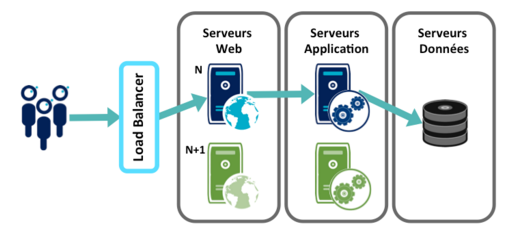
\includegraphics[scale=0.7]{images/BlueGreenDeployment.png}
          \end{center}
          \caption{Schéma du pattern « Blue/Green Deployment »}
          \label{BlueGreen}
        \end{figure}

        Une fois le déploiement effectué, notre nouvelle version doit être testée par une population restreinte d’utilisateurs. Le « Canary Release » confronte la version N+1 à une niche d’utilisateurs cibles tandis que la version N reste accessible à la majorité des utilisateurs (Voir Figure \ref{CanaryRelease}).\\

        \begin{figure}
          \begin{center}
            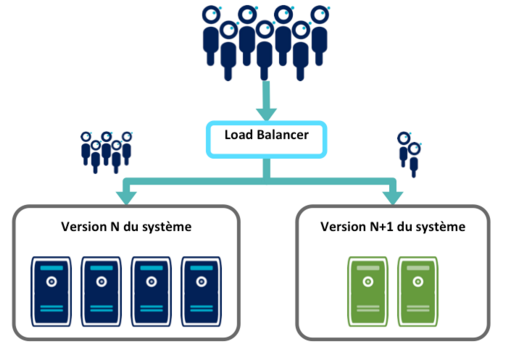
\includegraphics[scale=0.6]{images/CanaryRelease.png}
          \end{center}
          \caption{Schéma du pattern « Canary Release »}
          \label{CanaryRelease}
        \end{figure}

        La dernière étape du ZDD est le test de charge de notre nouvelle application. Le « Dark Launch » stimule progressivement le traffic généré par l’utilisateur afin de valider les performances et la scalabilité de notre plateforme. La stimulation progressive du traffic permet de préparer et d’optimiser au mieux notre plateforme afin que la mise en production finale de notre application se déroule sans problème.

        \subsubsection{La mise en oeuvre}
        Le point clé du ZDD est d'associer le mécanisme de répartition de charge (Load Balancer) à la cinématique de déploiement. Cette mise en oeuvre s'articule autour de trois grands temps (Voir Figure \ref{LoadBalancer}):\\

        \begin{itemize}
          \item le load balancer déconnecte de une à x chaine(s) de production sur laquelle est déployée la version N+1,
          \item une fois cette migration effective, le load balancer dirige une partie de ses utilisateurs vers cette nouvelle chaine contenant la version N+1,
          \item si la version N+1 est validée, la chaine de production en version N est déconnectée, mise à jour et reconnectée à la répartition de charge.\\
        \end{itemize}

        \begin{figure}
          \begin{center}
            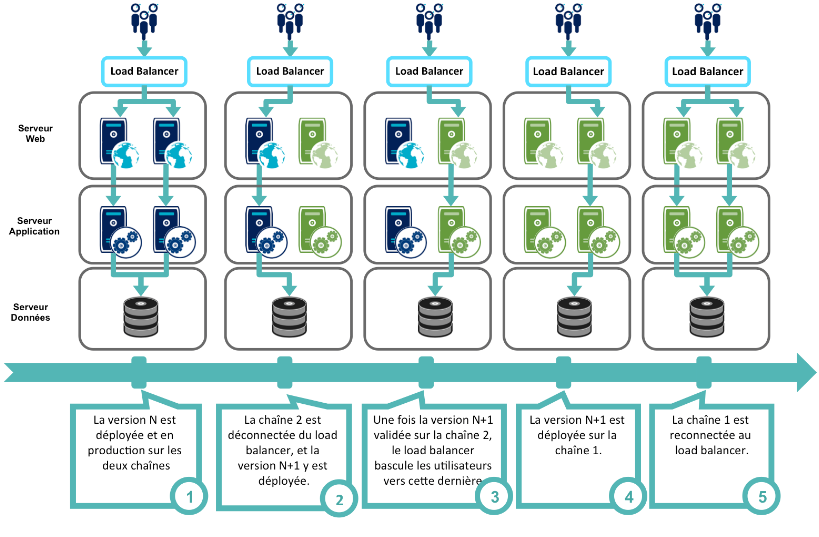
\includegraphics[scale=0.6]{images/LoadBalancer.png}
          \end{center}
          \caption{Schéma de la mise en oeuve du « Zero Downtime Deployment »}
          \label{LoadBalancer}
        \end{figure}

      \subsection{Le « Feature Flipping »}
      Les organisations appuyant leur service de livraison de code sur le Déploiement Continu se sont rapidemment confronté à une limite; comment commiter fréquemment sur le référentiel de source tout en garantissant la stabilité de l’application, toujours prête pour la production dans le cadre de fonctionnalités longues et complexes ? Deux possiblités s'offrent aux développeurs; créer une branche parallèle au niveau du référentiel de code et la maintenir ou créer une branche au niveau du code, le « Feature Flipping ».\\
      Le « Feature Flipping » permet d'activer ou de désactiver des fonctionnalités de l'application à chaud - directement en production sans relivraison de code. Le mécanisme est très simple, il suffit de conditionner l'exécution du code de la fonctionnalité avec un « if » qui ira regarder dans un fichier de configuration ou d'interroger une base de données afin de savoir si la fonctionnalité est activée ou non.\\

      Ce pattern offre trois axes d'amélioration aux applications:\\

      \begin{itemize}
        \item \textbf{sécuriser le déploiement}: l'activation et la désactivation d'une fonctionnalité à chaud permet d'éviter un processus de rollback,
        \item \textbf{expérimenter pour améliorer le produit}: il est possible d'étendre le « Feature Flipping » à une sous population d'utilisateurs, et en fonction de leur retour d'expérience activer la fonctionnalité ou non à l'intégralité des utilisateurs,
        \item \textbf{offrir un produit « customisable »}: il peut s'avérer intéressant à un moment du développement de laisser le choix à l'utilisateur entre deux modes de fonctionnement pour une même fonctionnalité.\\
      \end{itemize}


  \chapter{Implémentation - Etude de l'art}

  \section{Choisir ses outils}
  Une Plate-forme d'Intégration Continue (PIC) peut être mise en place avec un nombre incalculable d'outils différents. Il est important de comprendre la finalité et les caractéristiques de l'Intégration Continue que l'on souhaite mettre en place afin de choisir au mieux ses outils. L'Intégration Continue de base, peut être mise en oeuvre avec un ensemble très simple d'outils maisons mais généralement dans un environnement d'entreprise il est préférable d'utiliser les outils adoptés et soutenus par la communauté.

    \subsection{Scaling}
    Comme nous l'avons vu dans la section~\ref{Features of Continuous Integration}, l'Intégration Continue peut être mise en oeuvre en utilisant uniquement le contrôle de version, les scripts de build, un appel périodique à ces derniers et les emails. Cela peut s'avérer suffisant pour un projet simple, composé de quelques éléments, mais lorsque la quantité des composants buildables augmente cela peut dévenir un veritble cauchemar du côté de la maintenance. Pour résoudre ce problème de mise à l'échelle, un bon serveur d'Intégration Continue est indispensable. L'utilisation et la configuration d'un serveur d'Intégration Continue fourni par une société tierce est une tâche relativement triviale grâce à l'interface utilisateur graphique (\gls{GUI}) mise à la disposition des développeurs.\\

    Lorsque le nombre de builds, la quantité de code à compiler et le nombre de tests à exécuter augmentent, la puissance de calcul nécessaire augmente parallèlement. Afin d'accroitre la puissance de traitement de notre serveur d'Intégration Continue, on peut étendre, dans certaines limites, la quantité de coeurs de son processeur (CPU) - scalabilité verticale - ou augmenter le nombre de serveurs physiques dédiés à la PIC - scalabilité horizontale. Cette scalabilité horizontale est aussi nécessaire lorsque que la build à besoin de s'exécuter sur différents environnements ou plates-formes.

    \subsection{Le choix du serveur d’Intégration Continue}

      \subsubsection{Support du langage de programmation}
      Il existe divers serveur d'Intégration Continue, chacun porté par une entreprise informatique différente. Certains d'entre eux sont conçus pour ne fonctionner qu'avec des langages de programmation spécifiques tandis que d'autres sont génériques et fonctionnent avec tous. Si l'entreprise dispose d'un parc informatique uniforme dans le langage et ne compte en déroger la première option peut être viable dans le cas contraire l'entreprise devra se tourner vers un serveur d'Intégration Continue générique.

      \subsubsection{Support du référentiel de code source}
      De même que pour le langage de programmation, le support du référentiel de code source doit être pris en compte lors du choix du serveur d'Intégration Continue. Nous distinguons deux mécanismes de communication entre le référentiel et le serveur; les Agents et les Webhooks.\\

      Les agents sont des modules, intégrés (dans le cadre d'un serveur propriétaire) ou non (dans le cadre de l'open source), qui effectuent, en toute transparence pour l'utilisateur, le lien entre le référentiel et le serveur. Leur utilisation est extrèmement simple et ne nécessite que très peu de configuration. L'inconvénient des agents est que si votre gestionnaire de code source n'est pas pris en compte, il est dès lors impossible d'utiliser ce serveur avec votre référentiel dans le cas d'un logiciel propriétaire ou très coûteux de développer votre propre agent dans le cas d'un serveur d'Intégration Continue open source.\\

      La majorité des serveurs d'Intégration Continue proposent un second mécanisme de communication avec le référentiel de code source via les Webhooks. Les webhooks servent à notifier des éléments externes à une application web qu'un événement a eu lieu sur celle-ci. Les serveurs d'Intégration Continue s'assurent ainsi d'être agnostiques du référentiel. Cependant votre gestionnaire de code source doit lui aussi implémenter les Webhooks pour pouvoir notifier le serveur.

      \subsubsection{La gestion des builds}
      Un des points importants à prendre en compte lors du choix de son serveur d'Intégration Continue est sa gestion des builds. Le déclenchement des builds, la possibilité d'exécutions parallèles, la gestion des dépendances interprojets, etc, sont propres à chaque serveur. Il est intéressant d'étudier chacune de ces spécificités afin de choisir l'outil le plus adéquat à vos besoins.

      \subsubsection{Extensibilité}
      Dans le cas ou aucun serveur d'Intégration Continue ne répond par défaut à l'intégralité de vos besoins, un serveur qui peut être étendu avec des plugins se révèle être un bon choix. Avec ce mécanisme de plugin, pratiquement tout outil peut être intégré. Vous trouverez sur internet une quantité de plugin en fonction de votre serveur d'Intégration Continue. Vous êtes aussi libre de créer le votre et de le proposer à la communauté.

      \subsubsection{Autres caractéristiques}
      Les serveurs d'Intégration Continue ont un large éventail de caractéristiques que nous n'avons pas encore abordé mais qui doivent être pris en considération lors de votre choix.
      \paragraph{La publication} La publication regroupe la création des rapports et des artefacts ainsi que leur gestion. La méthode de base pour publier est l'email. Certains serveurs supportent également le Secure Copy (SCP), le protocole de transfert de fichier (\gls{FTP}), les flux RSS...
      \paragraph{L'interface utilisateur} La caractéristique la plus visible des serveurs d'Intégration Continue est son interface utilisateur. La tendance est d'avoir une interface web. Rassurer-vous tous les serveurs en proposent une, ce qui fait la différence est, ce qui peut être fait à travers elle.
      \paragraph{Le suivi de problèmes} Si vous utilisez un outil de suivi de problèmes tel que Jira ou Bugzilla vous pouvez l'intégrer directement dans votre serveur d'Intégration Continue, dans la mesure ou votre serveur dispose d'un agent ou d'un plugin à ces effet.
      \paragraph{L'environnement de développement} Certains serveurs d'Intégration Continue peuvent être intégrés aux environnements de développement (IDE). Pour cela votre IDE doit disposer d'un plugin pour votre serveur. Avec de tels plugins les statuts de vos builds peuvent être vus directement à partir de l'IDE sans avoir accès à l'interface graphique de votre serveur.

      \subsubsection{Installation et configuration}
      Un serveur d'Intégration Continue peut être installé de multiple façons. Pour les environnements Windows, presque tous les serveurs fournissent un installateur qui exécutera toutes les mesures nécessaires afin que vous disposiez d'une installation fonctionnelle. Pour les autres environnements les serveurs d'Intégration Continue soumettent des distributions autonomes telles que les paquets Debian ou les Web Archive (WAR). Dans ce cas, avant toute installation, vous devez vérifier les dépendances additionnelles (sdk, framework, ...) mentionnées dans le guide d'installation.\\

      Une fois l'installation effectuée le serveur d'Intégration Continue doit être configuré. La plupart des serveurs fournissent une interface graphique pour cela. Vous devrez en outre définir l'emplacement et le type de votre référentiel de code source, les outils de build, les contrôles d'accès... L'intégralité des serveurs, même ceux possédant une interface graphique, sauvegarde vos configurations dans des fichiers ou dans des bases de données. Votre configuration peut ainsi être archivée, partagée et réutilisée.

      \subsubsection{Autres questions à considérer}
      \paragraph{Les coûts} Les coûts de mise en place et de maintenance du serveur d'Intégration Continue sont un point à prendre en compte lors de votre choix. Il existe des serveurs gratuits - open source - (Jenkins) et des serveurs payants - propriétaire - (Visual Studio Team Services). Les serveurs open source sont libres d'utilisation mais ne proposent bien souvent pas de support technique. A l'inverse les serveurs payants nécessitent une licence d'utilisation mais fournissent un support technique, une expertise ainsi qu'un accompagnement.

      \paragraph{La communauté} Les serveurs d'Intégration Continue largement diffusés disposent d'une forte communauté active. Les solutions aux problèmes d'installation et de configuration courants sont généralement disponibles sur internet. De plus une communauté active pourra répondre à vos questions spécifiques. Une bonne communauté en ligne peut être une substitution aux supports techniques.

  \section{Logiciels et outils utilisés au sein de la DSI d'AXA France}
  Depuis maintenant 3-4 ans la DSI d'AXA France dispose d'une équipe dédiée à la mise en place, la maintenance et l'accompagnement des équipes dans l'Intégration Continue. Encore en phase de développement seuls quelques projets bénéficient de cette évolution. Dans la suite de ce mémoire nous prendrons en compte que les langages prédominants dans le parc applicatif d'AXA qui sont le Java, le C\# et le Javascript.

    \subsection{Serveur d’Intégration Continue}
    Historiquement, au sein d'AXA, deux grands langages composent essentiellement l'ensemble du socle applicatif web de l'entreprise; le Java (J2EE) et le C\# (.NET). Le choix du groupe s'est tourné vers l'utilisation de deux serveurs d'Intégration Continue distincts. Un serveur basé sur la suite Microsoft Visual Studio Team Services (\gls{VSTS}) pour les applications .NET et un serveur basé sur le produit open source Jenkins pour les applications J2EE, Javascript ...\\

    De par son background informatique, AXA est attaché aux solutions proposées par Microsoft. La synergie des technologies Microsoft et son support technique offrent aux entreprises une garantie non négligeable quant à la qualité de ses services. C'est tout naturellement qu'AXA s'est dirigé vers leur serveur d'Intégration Continue Visual Studio Team Services 2010 pour les applications liées à l'environnement Microsoft - applications développées en .NET et déployées sur des serveurs Windows. Cependant, la version de VSTS 2010 ne supportait pas l'intégration et le déploiement de langages autres que ceux portés par Microsoft (depuis la version 2015 si). AXA a donc dû se tourner sur une autre solution pour le reste de ses applications.\\

    Jenkins est le leader des serveurs d'Intégration Continue open source. Développé en Java, il peut aussi bien être déployé dans un environnement Windows que Linux. De plus Jenkins et sa communauté proposent une pléthore de plugin afin d'intégrer facilement Jenkins dans votre environnement de travail. AXA s'est donc orienté vers cette solution pour ses applications Java et Javascript. Mais si Jenkins fournit les plugins nécessaires à l'intégration et au déploiement des applications .NET, pourquoi AXA propose la solution VSTS à ses équipes C\#?\\

    Jenkins est un produit développé en Java et open source, dans la plupart des cas il est installé sur un serveur Linux et configuré via son interface web administrative. Les applications destinées aux serveurs Linux peuvent être déployées sans problème. Toutefois, si votre application requiert une compilation .NET le problème se corse. La communauté met à disposition le plugin MSBuild pour palier à ce problème. Cependant celui-ci requiert une dll (du même nom) et étonnamment Microsoft ne propose pas de distribution Linux pour cette dernière. Il est toujours possible d'exécuter la dll MSBuild avec une surcouche WINE ou Mono mais le défis technique se révèle être une perte de temps dans la plupart des cas.
    Une alternative serait d'installer Jenkins sur un serveur Windows, et dans ce cas aucun problème d'intégration et de déploiement du côté des applications .NET. Nous aurions ainsi une PIC unique pour toutes nos applications. Néanmoins AXA a pour volonté de rester dans un écosystème Microsoft pour les applications .NET. Nous nous retrouvons ainsi avec 2 plate-formes d'Intégration Continue, une tournant sur Visual Studio Team Services 2013 et une sur Jenkins 1.2.\\

    \begin {boxedminipage} {11cm}
      Dans la suite de ce mémoire nous étudierons exclusivement la plate-forme d'Intégration Continue basée sur Jenkins.
    \end {boxedminipage}\\

    \subsection{Logiciel de gestion de version}
    Au moment ou j'écris ce mémoire, une grande migration du référentiel de code source a lieu à AXA. L'ancien outil, ClearCase - propriété d'IBM - est abandonné au profit de Team Foundation Server (\gls{TFS}) - propriété Microsoft. Toutes les nouvelles applications, et donc celles impactées par l'Intégration Continue, ont officiellement pour gestionnaire de version cible TFS. Cependant quelques projets sont hébergés sur d'autres référentiels de code source, tel que BitBucket (Atlassian), lors de leur développement et archivés sur TFS une fois en production.

    \subsection{Outils de build}
    Les outils de build sont intrinsèques au langage de programmation. Pour le Java nous utilisons Maven, intégré dans Jenkins et pour le Javascript Grunt ou Gulp - en fonction des équipes de développement - associé à Jenkins via des plugins.

    \subsection{Analyse statique du code}
    Afin d'uniformiser et d'améliorer la qualité de l'ensemble des morceaux de code source synchronisés par chaque développeur, AXA a intégré à sa plate-forme d'Intégration Continue SonarQube, un outil d'analyse de code. Il couvre notamment l'architecture et le design, la complexité, la duplication de code, les normes de développement, les bugs potentiels, les tests unitaires, etc (Voir Figure \ref{SonarQube}). Initialement développé pour analyser le Java, de nombreux plugins offrent la possibilité d'étendre SonarQube aux autres langages de programmation. SonarQube analyse votre code et lui accorde une note (en pourcentage) permettant ainsi de rejeter les commits ne satisfaisant pas les seuils fixés.\\

    L'intégration d'un analyseur statique de code au sein du serveur d'Intégration Continue et d'un pipeline de déploiement est rendu possible par le biais de plugins développés par la communauté Jenkins.

    \begin{figure}
      \begin{center}
        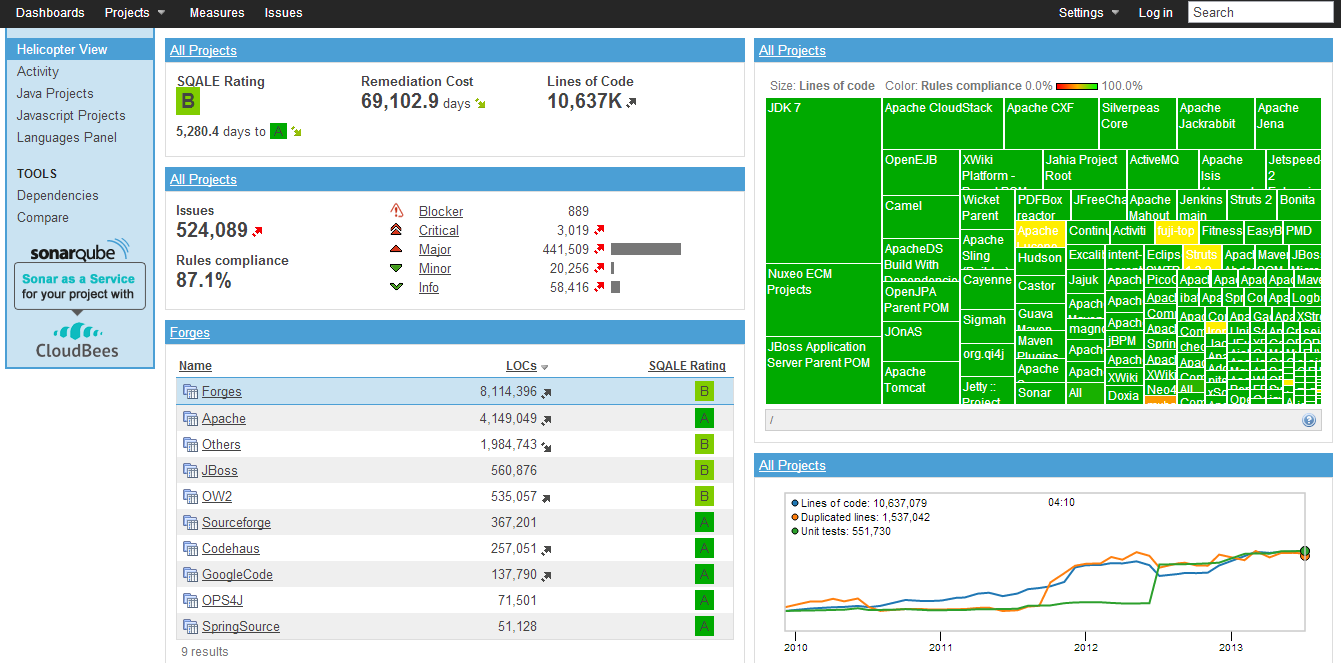
\includegraphics[scale=0.3]{images/SonarQube.png}
      \end{center}
      \caption{Exemple d'un rapport d'analyse statique de code fournit par SonarQube}
      \label{SonarQube}
    \end{figure}

    \subsection{Automatisation des tests et de la couverture de code}
    L'exécution des tests, par le biais de framework, est propres à chaque langage et à chaque équipe de travail. En javascript par exemple, les tests unitaires peuvent être mises en place avec Moccha, Jasmine, Unitjs... Le serveur d'Intégration Continue ne fait qu'automatiser leur lancement à chaque commit du code source et disposer d'un affichage graphique des résultats via le plugin JUnit Plugin. Pour cela le framework de test doit fournir en sortie un rapport au format XML (Voir Figure \ref{ReportXML}) qui sera interprété par le plugin JUnit.

    \begin{figure}
      \begin{center}
        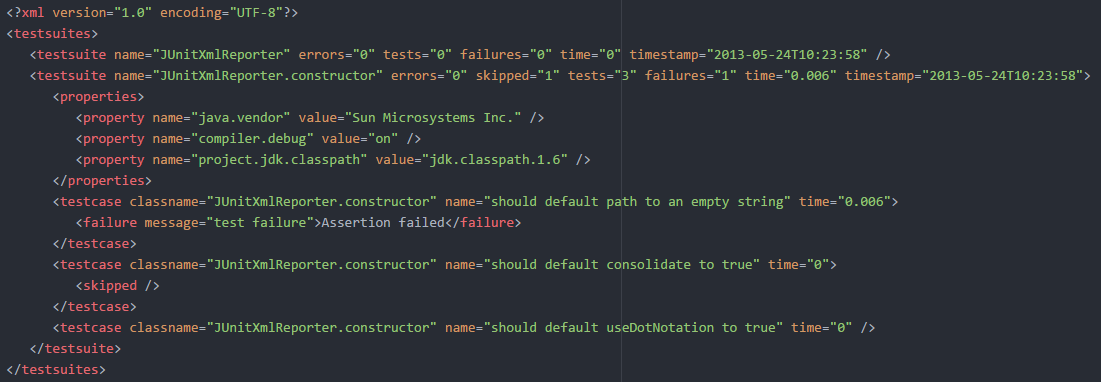
\includegraphics[scale=0.5]{images/ReportXML.png}
      \end{center}
      \caption{Exemple d'un rapport de test au format XML d'une application Java}
      \label{ReportXML}
    \end{figure}

    \subsection{Documentation Continue}
    Les équipes de développement d'AXA ne sont soumis à aucune politique de documentation du code source. Libre à chacun de documenter ou non son développement. De ce fait, la Documentation Continue ne fait pas partie des fonctionnalités de notre plate-forme d'Intégration Continue.

    \subsection{Déploiement Continu}
    Officiellement AXA possède quatre environnements dans le cycle de de développement d'une application; l'environnement de développement, l'environnement de recette (ou de qualification), l'environnement de pré-production et celui de production. De plus la DSI d'AXA France subit une profonde transformation digitale poussée par l'émergence du Cloud. Une forte volonté de migration des applications AXA dans le cloud est présente. Cependant la migration étant longue et encore en phase de test, peu d'applications sont hébergées dans le Cloud ce qui implique le maintient d'une infrastructure physique. Le Déploiement Continue au sein d'AXA doit donc prendre en compte 4 environnements ainsi que deux types d'architectures serveur.\\

    L'infrastructure serveur de la DSI d'AXA est gérée par un prestataire de service interne à AXA - AXA Tech. Les développeurs n'ont ainsi qu'une très faible marge d'action sur la gestion des divers environnements. Le Déploiement Continue est ainsi possible sur les trois premiers environnements (développement, recette, pré-production). Le déploiement sur les instances de production est fait manuellement lors de mises en production (\gls{MEP}) éparses.\\

    L'utilisation de la technologie des conteneurs (Voir la section \ref{Containers}) n'est encore que trop peu développée au sein d'AXA faute de non compatibilité des serveurs.

      \subsubsection{La gestion des dépendances}\label{Nexus}
      Lors du développement d'une application de nombreuses dépendances sont utilisées. A AXA, la gestion de ces dernières est effectuée par le gestionnaire de dépendance (ou repository manager) Nexus, qui permet de répondre à deux problématiques; il agit comme un proxy entre AXA et les dépôts publics et permet d'organiser la localisation des déploiements des dépendances spécifiques à l'entreprise.\\

      Fournir un proxy (et en même temps un cache) aux dépôts publics distants permet d'accélerer le processus de build en évitant le téléchargement redondant des dépendances. Les dépendances ne seront téléchargées qu'une unique fois depuis internet et stockées au niveau du cache du repository manager. De plus il permet à l'organisation de contrôler les dépendances téléchargées ainsi que leur version, garantissant une uniformité des ces dernières.

      Le repository manager a aussi pour fonctionnalité de mettre à la disposition de l'entreprise un dépôt interne partagé où les binaires et autres artefacts générés peuvent être entreposés et versionnés.\\

    \subsection{Feedback Continue}
    Notre plate-forme d'Intégration Continue Jenkins utilise les emails comme chaine de rétroaction primaire. Les rapports par mail sont très faciles à mettre en place. Du côté de la configuration, Jenkins envoie des emails après chaque build échouée et en cas de changement d'état de construction. Nous avons également inclus l'identité du dernier développeur à avoir cassé ou réparé la build afin de favoriser la collaboration des divers acteurs. Les adresses mails des bénéficiaires sont prédéfinies et les équipes de travail sont détermineées afin de faciliter la gestion de la rétroaction par email.\\

    Nous utilisons l'interface web de Jenkins comme chaine de feedback secondaire. Hautement disponible, elle fournit l'intégralité des données nécéssaires à à la rétroaction et permet aux équipes d'avoir une vue générale de l'état des différentes builds de leurs applications.

  \section{Architecture}

    \subsection{Serveur d’Intégration Continue}
    Notre serveur d'Intégration Jenkins est déployé sur une ferme de serveurs composée d'une instance maître (Master), installée sur un RedHat 6.5 (Linux) et de plusieurs serveurs esclaves (Slaves); deux instances sur MacMini pour les applications mobiles IOS/Android et N instances sur Solaris (Linux) pour toutes les autres applications. Cette architecture Master/Slaves est transparente pour les utilisateurs. Ils intéragissent uniquement avec l'instance maître. Le Master donne les ordres, les Slaves les exécutent. Ce modèle permet en autre d'accroître la puissance de notre serveur Intégration Continue en s'appuyant sur la scalabilité horizontale, qui rappelons le, améliore les performances en ajoutant de nouveaux serveurs (en opposition à la \gls{scalabiliteverticale} qui elle repose sur une amélioration de la puissance du serveur).

    \subsection{Logiciels de gestion de configuration}
    Les logiciels de gestion de configuration, qu'ils agissent sur le code source ou sur les artefacts (Nexus), sont déployés sur des serveurs spécifiques et disposent de serveurs de réplications afin de palier à tout dysfonctionnement.

    \subsection{Outils de build}
    Les divers outils nécessaires à la build sont soient hébergés directement sur les serveurs d'Intégration Continue (outils de compilation, de tests unitaires, ...) soient ils disposent de leur propre instance (outils d'analyse de code, de test d'intégration, de test d'intrusion, ...).

    \subsection{Réseaux et déploiement}
    L'intégralité des composants de la PIC Jenkins étant hébergé dans les datacenters d'AXA, la communication entre eux s'effectue via le réseau interne d'AXA (intranet). Aucun n'accès externe n'est possible.\\

    Le Déploiement Continue à AXA repose sur quatre types de serveurs cibles, en fonction de la nature des artefacts buildés - sans compter leurs divers environnements (développement, recette, pré-production, production). La première famille de serveur, utilisé pour les applications en « \gls{authoring} »\footnote{Authoring: solution qui permet à ses utilisateurs de créer des applications multimédia pour manipuler des objets multimédias tels que les blogs, les sites d'information...}, repose sur Adobe Experience Manager (\gls{AEM}). Techniquement, AEM est une application serveur fonctionnant sous la plateforme Java SE sur Windows, Mac ou Unix et accessible depuis un navigateur Web. Un site peut être sauvegardé sous la forme d’un package Zip et ensuite être déployé avec une grande simplicité sur d’autres environnements.\\

    Le deuxième type d'instance, les serveurs NodeJS, correspond aux applications Javascript. Le déploiement, l'installation et la configuration des artefacts s'effectuent via le protocole de communication sécurisé SSH et le Node Package Manager (\gls{npm}), le gestionnaire de paquet propre aux Javascripts, connecté à notre repository/proxy Nexus.\\

    Les applications Android/IOS sont quant à elles déployées sur des serveurs hébergeant HockeyApp, un outil Microsoft permettant de tester les versions béta des applications mobiles. Le déploiement s'effectue par le push direct des .apk et .api (respectivement les artefacts Android et IOS) sur HockeyApp.\\

    Le quatrième et dernier type d'instance concerne les applications Java. Il s'appuie sur le système d'exploitation Solaris (Linux) et le serveur web Tomcat. Le déploiement se réalise par l'exécution direct des scripts issues de la build et déployant les .war (artefact J2EE) sur les instances cibles.

    \begin{figure}
      \begin{center}
        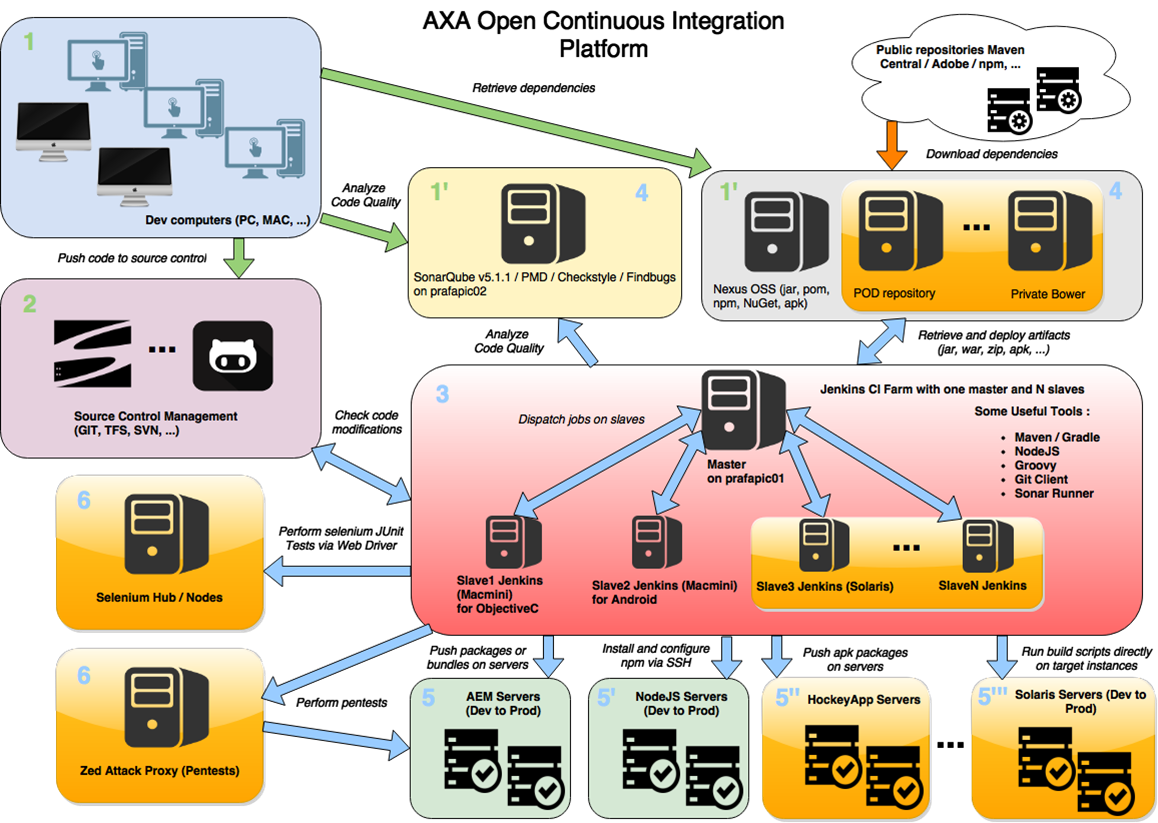
\includegraphics[scale=0.5]{images/PICJenkins.png}
      \end{center}
      \caption{Schéma d'architecture de la Plate-forme d'Intégration Continue Jenkins}
      \label{PICJenkins}
    \end{figure}

  \section{Configuration}

    \subsection{« Build Jobs »}

      \subsubsection{Découpage des jobs}
      Plus l'exécution d'une build est longue, plus le temps de la rétroaction augmente. Or un des objectifs de l'Intégration Continue est de minimiser cette rétroaction. Cinq minutes, est le seuil maximal défini par AXA pour la réalisation d'un Job. Si un Job prend plus de temps, il est nécessaire de la découper en plusieurs étapes consécutives. Jenkins est designé pour permettre le déclenchement des Jobs les un après les autres. Il est donc facile de détailler une construction lourde en plusieurs petites étapes, favorisant la rétroaction après chaque étape sans avoir à attendre la fin de la construction. \\

      Nous ne pouvons pas définir de découpage générique à toutes les applications présentes dans la PIC AXA; trop de paramètres entrent en compte. En revanche nous pouvons décrire une séquence type, illustrative d'un worflow d'Intégration Continue. Les jobs s'exécutant séquentiellement si et seulement si le précédent est un succès. Le premier Job lancé est l'inspection statique du code source, suivi de la compilation, des tests, du packaging et du déploiement. Les tests, de par leur temps d'exécution, sont eux aussi découpés en plusieurs Jobs. Les tests unitaires, étant la première couche dans la hiérarchie des tests et la plus rapide à exécuter, ouvrent le bal.

      \subsubsection{Etablir des relations}
      Le déclenchement séquentiel des Jobs, les uns après les autres, peut également être utilisé pour gérer les dépendandes de construction. Si un module logiciel A dépend d'un module B et C, la construction de A peut être déclenchée si la build d'une des dépendances est exécutée. Jenkins met en place un mécanisme d'upstream (amont) et de downstream (aval) pour les relations de dépendance. Quelques fois les équipes de développement effectuent plusieurs commits sur un module logiciel unique dans un court laps de temps, afin de diviser l'intégration en petits lots commentés. En pratique tous ces commits peuvent être interprétés comme un seul. Pour éviter le déclenchement de builds upstream ou downstream Jenkins introduit une période de silence. Si une build est configurée pour avoir cinq minutes de période de silence, elle est mise en attente lorsqu'elle est déclenchée et ne s'exécute que si aucun autre commit à eu lieu sur le module pendant ce laps de temps. Sinon la période de silence est de nouveau repoussée à cinq minutes.\\

      Jenkins peut également être configuré pour éviter les déclenchements downstream (aval) des builds pendant l'exécution d'une build upsteam (amont).

    \subsection{Reporting}
    Pour chaque build nous générons automatiquement différents rapports à l'aide des fonctionnalités et plugins intégrés à Jenkins. Nous recueillons ainsi les résultats des tests et de la couverture de code (pour les tests unitaires). D'après les résultats, l'interface web de Jenkins génère des graphiques de tendance, qui visualise la quantité de tests passants et non-passants au fil du temps (Voir la Figure \ref{JenkinsTestReport}). Il est également possible de visualiser les résultats d'un test particulier. AXA configure ses builds pour conserver un historique sur trente exécutions.\\

    \begin{figure}
      \begin{center}
        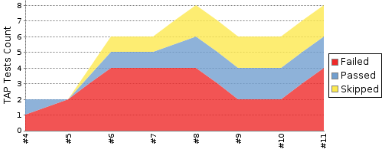
\includegraphics[scale=1]{images/JenkinsTestReport.png}
      \end{center}
      \caption{Exemple d'un graphique de tendance des tests unitaires dans Jenkins}
      \label{JenkinsTestReport}
    \end{figure}

    Les violations de conventions de codage sont également enregistrées. Avec le plugin adéquat, le rapport présenté dans Jenkins nous montre visuellement le nombre de violations ayant eu lieu ainsi que leur gravité (Voir la Figure \ref{JenkinsCodingReport}). Nous disposons même d'une vue de navigation où les lignes en violation sont surlignées dans le code source.\\

    \begin{figure}
      \begin{center}
        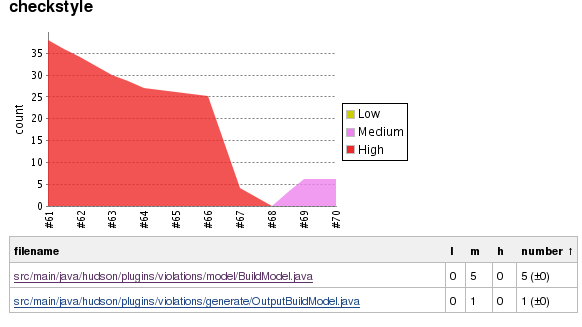
\includegraphics[scale=0.7]{images/JenkinsCodingReport.png}
      \end{center}
      \caption{Exemple d'un graphique de violation de convention de codage dans Jenkins}
      \label{JenkinsTestReport}
    \end{figure}

    La complexité du code source est également inclue dans les rapports de construction, permettant un refactoring rapide et garantissant une qualité de code.

  \section{Délivrables et artéfacts de build}
  Le type de délivrable attendu dépendra essentiellement du langage de l'application, de votre infrastructure et de la politique de déploiement de votre compagnie. Chez AXA, les applications Java sont packagées en war, les applications .NET en msi et les applications Javascript en zip. Les containeurs ne sont pas encore utilisés au sein d'AXA, faute de non compatibilité de nos serveurs. L'intégralité de ces artefacts est archivé et versionné dans notre repository manager \gls{Nexus} (dans le cadre de notre PIC Java/Javascript, pour la PIC .NET nous utilisons TFS).\\

  Ces délivrables sont nos principaux artéfacts de build, mais notre Intégration Continue produit également de la documentation, des changelogs et des rapports de build (vus dans la section précédente). En fonction de leur nature ils sont archivés et versionnés directement dans notre gestionnaire de code source ou dans Jenkins.\\

  \section{Observations et conclusion}
    \subsection{Point de départ}
    Avant la mise en place de l'Intégration Continue à AXA il n'y avait pas de processus abordant l'assurance de la qualité à tout niveau. La responsabilité de celle-ci était à la charge du développeur, dictée par son professionnalisme et sa motivation. Il était à la décision de chacun de tester son application avant qu'elle ne soit mise en production. Les étapes de compilation, de packaging et de déploiement étaient manuelles, ce qui demandait une charge de travail rébarbative et source d'erreurs pour les équipes de développement. Les déploiements étaient sporadiques et trop éloignés dans le temps conduisant à des mises en production douloureuses. C'est autant plus éprouvant éprouvant, que pour la mise en production, les équipes de travail d'AXA doivent passer par AXA Tech, le prestataire interne de notre infrastructure.\\

    \subsection{Les méthodes de travail}
    La majorité des développeurs présents à AXA ont eu une expérience de travail sans Intégration Continue. Le passage à l'Intégration Continue a changé leur façon de travailler et pour beaucoup d'entre eux avec un impact bénéfique. Même les développeurs qui n'étaient pas au courant de l'intégralité des règles de l'Intégration Continue vu dans la section \ref{Developers} ont pu facilement s'adapter à cette nouvelle méthodologie de travail; cela étant dû à leur bon sens.

      \subsubsection{Commiter les changements}
      Tous les développeurs passés à l'Intégration Continue synchronisent au moins quotidiennement leur changement avec le dépôt de code source. Leur fréquence depend de la tâche sur laquelle ils travaillent. S'ils développent une nouvelle fonctionnalité la fréquence d'intégration est plus faible que s'ils résolvent un bug ou effectuent une réfactorisation. Leur fréquence de commit correspond aux tâches agiles qu'ils effectuent - une tâche entraine irrémédiablement un commit.

      \subsubsection{Les tests locaux}
      L'une des étapes du cycle de travail de l'Intégration Continue est d'exécuter localement les tests avant d'intégrer leurs changements au dépôt partagé. Cependant nous constatons que certains développeurs n'exécutent les tests en local que lors de l'échec de leur build, pensant à tord que leur exécution par le serveur d'Intégration Continue les en dispense. Dans d'autre cas, les développeurs ne sont pas en mesure d'effectuer les tests en local ne disposant pas de l'environnement nécessaire.

      \subsubsection{Usage des rapport et de la rétroaction}
      L'un des avantages de l'Intégration Continue est d'améliorer la visibilité des problèmes liée à la construction de artefacts de l'application (Voir la section \ref{Benefits}). Toutes les personnes que j'ai pu interroger ont indiqué qu'il était facile de trouver les informations liées à la santé d'une build. Les informations sont centralisées et standardisées au niveau du serveur d'Intégration Continue. Le point le plus intéressant de ces rapports et l'état général des constructions - échec ou succès. En cas d'échec le premier rapport est fourni par le message de sortie de la console du serveur.\\

      Les rapports de tests générés sont généralement peu utilisés car ils nécessitent une navigation au travers de plusieurs écrans tandis que la même information est présente dans le rapport précédent.\\

      Les rapports de code des analyseurs statiques sont très utiles aux développeurs. Ils standardisent les morceaux de code de chacun, renseignent sur les besoins de refactoring, et indiquent l'absence de documentation.\\

      Les retours par emails effectués par le serveur d'Intégration Continue sont généralement suivis même si quelques développeurs ont mentionné le fait que l'email n'était, pour eux, pas une bonne solution. Certains ont classé ces emails comme spams tandis que d'autres consultent très peu leur boite de messagerie. Il a égalemment été évoqué que lorsqu'une build échoue, à cause d'un problème autre qu'une erreur de programmation (problème d'installation par exemple), le rapport ne stipule pas clairement que le code poussé par le développeur est correct. Ce genre de problème et le manque de robustesse dans les builds réduisent le profit de la rétroaction.\\

      En dépit des problèmes liés à la rétroaction, on constate que lorsqu'un problème a été identifié il est fixé rapidement.

      \subsubsection{Configuration des builds d'Intégration Continue}
      Les deux plate-formes d'Intégration Continue mise en place par AXA sont gérées exclusivement par une équipe dédiée. Ce qui pose problème à certaines équipes de développeurs qui souhaiteraient être maître de la configuration de leurs builds. De plus la demande de création et de configuration d'un pipeline de déploiement suit un processus lent et complexe composée d'une multitude d'intervenants ne favorisant pas l'agilité dans la création de projet. Ce qui induit que de nombreuses applications ne bénéficient pas encore de l'infrastructure nécessaire à la pratique de l'Intégration Continue.

    \subsection{Les bénéfices constatés}
    Le packaging automatique et le déploiement facile sont les principales caractéristiques de l'Intégration Continue. Réduire le workflow fastidieux du déploiement d'une application en une ligne de commande ou une action offre plus de temps libre aux développeurs qu'ils peuvent consacrer à des activités à valeur ajoutée (refactorer, imaginer, créer). Cela permet également de réduire les frustrations et d'augmenter ainsi la motivation des développeurs. Outre les bénéfices pour le développeur, l'automatisation améliore la qualité de l'intégration et de la livraison en évitant toute erreur d'inattention et en réduisant le temps de déploiement.\\

    L'intégralité des développeurs ont mentionné que l'un des principaux avantages de cette nouvelle méthodologie de travail est l'automation des tests. Pour chaque changement apporté au code source la totalité des tests sont exécutés et si ne serait-ce qu'un test se révèle être défaillant aucun nouveau package ne sera créé et le code poussé ne sera pas incorporé au code source partagé. Les problèmes sont ainsi déclarés rapidemment et n'impactent qu'un seul développeur. La propreté et la qualité du code source sont garanties par l'Intégration Continue.\\

    Un autre bénéfice constaté est la gestion des builds de « développement » et de « release ». Le serveur d'Intégration Continue, grâce à ses plugins, marque les différents artefacts produits en fonction de leur version et de leur environnement. Cela permet de conserver un historique des builds et d'éviter l'installation de mauvais packages.\\

    \subsection{Les axes d'amélioration}
    La PIC Jenkins, quoique remplissant son rôle, n'est pas parfaite. Le premier axe à prendre en compte est son aspect centralisé. Les équipes de développement ont uniquement les droits d'exécution et ne peuvent ainsi interagir dans la personnalisation de leurs pipelines de déploiement. Une équipe spécialisée est chargée de la configuration et de la gestion des Jobs pour l'ensemble de l'organisation. Victime de son succès l'Intégration Continue fait de plus en plus d'adepte au sein d'AXA, ce qui accroît la demande au niveau de la PIC. Les délais de disponibilité des nouveaux Jobs, parfois longs, continuent d'augmenter, ce qui nuit fondamentalement à la philosophie de l'Intégration Continue.\\

    Techniquement l'utilisation de deux technologies implique la maintenance de deux plateformes, pour un résultat similaire. cette différence engendre également des coûts supplémentaires, des coûts financiers mais aussi de temps et de ressources humaines. Il serait intéressant de fusionner les PIC Java/Javascript et .NET afin de ne disposer que d'un seul type d'infrastructure.\\

    Avec l'essor du Cloud, un autre axe d'amélioration serait de « cloudifier » nos plate-formes d'Intégration Continue afin de bénéficier du concept ATAWAD - « AnyTime, AnyWhere, AnyDevice » (tous le temps, depuis n'importe où, sur n'importe quel device) - et de réduire les coûts d'infrastructure.\\

    D'après les temoignages de développeurs travaillant en Intégration Continue sur les PIC AXA, la rétroaction des builds par email et par l'interface du serveur ne correspond pas à leurs attentes. La communication entre les collaborateurs et l'outil d'Intégration est un axe à améliorer.


  \chapter{Amélioration - Codé, Automatisé, Générique, Open Source et dans le Cloud}

  \section{Les objectifs de cette nouvelle plate-forme d'Intégration Continue}
  L'objectif principal de cette nouvelle plate-forme est avant tout d'assurer les fonctionnalités primaires de l'Intégration Continue vues dans la partie \label{ContinousIntegration} et déjà présentes dans la PIC Jenkins d'AXA.\\

  Le Cloud est le mot à la mode des dernières années au sein des organisations. L'idée principale derrière le Cloud est que vous pouvez accéder à l'intégralité de vos ressources sur Internet de n'importe où et à tout moment. De par la mobilité des équipes de travail et de l'internalisation des collaborateurs la solution Cloud peut être un réel atout dans la mise en place de notre solution. Un autre objectif à prendre en compte et étroitement lié au Cloud est l'automatisation du provisionnement et du déploiement de notre PIC. Dans l'idéal, l'installation et la configuration de notre serveur d'Intégration Continue ne devraient avoir besoin d'action humaine une fois le processus lancé.\\

  Un autre enjeux à prendre en compte est la généricité de notre solution. Elle doit être compatible avec l'ensemble des langages de programmation ainsi que des divers outils gravitant autour du développement, de l'intégration et du déploiement. Une PIC unique pour l'ensemble de l'organisation. Attention cependant, nous parlons ici d'une PIC unique dans architecture, son déploiement, son fonctionnement, son utilisation et non pas dans son identité et sa configuration.\\

  Depuis quelques temps, la Blockchain est le sujet qui agite de nombreux secteurs. Technologie permettant de décentraliser et désintermédier un nombre conséquent de processus et d’applications traditionnelles (banques, entreprises, administrations…), elle promet une révolution à de nombreux égards. Une des facettes les plus importantes, et pourtant peu abordée, de cette révolution annoncée, réside dans le changement de paradigme organisationnel, et permet d’envisager la fin des structures hiérarchiques traditionnelles. Ce nouveau paradigme répond très bien à notre problématique de PIC déscentralisée. Chaque équipe de développement serait responsable de son propre serveur d'Intégration Continue. Les plate-formes d'Intégration Continue seraient alors gouvernées par les acteurs du projet eux-mêmes. Couplés au Cloud et à l'automatisation de son déploiement, sa mise en place et sa prise en main permettrait à tous les développeurs de profiter des bénéfices de l'Intégration Continue.\\

  Un des objectifs de cette solution est d'offrir une plate-forme d'Intégration à tous les développeurs d'une organisation mais aussi et surtout de l'offrir à toutes les organisations, qu'elles soient petites, grandes, riches, pauvres... Propager l'Intégration Continue est une garantie dans l'amélioration de la qualité logicielle. Pour cela l'intégralité des outils utilisés doit être gratuite ou en libre utilisation.

  \section{Le serveur d’Intégration Continue}
  Afin de répondre à la problématique de la généricité de la plate-forme d'Intégration Continue et de l'open source, le serveur d'Intégration Continue devra répondre aux caractéristiques suivantes:\\

  \begin{itemize}
    \item multiplate-forme (Windows et Linux),
    \item multi-langage (.NET, JAVA/J2EE, Javascript, ...),
    \item multi-référentiel de code source (Git, TFS, SVN, ...),
    \item open source.\\
  \end{itemize}

    \subsection{Jenkins leader mais ...}
    Jenkins (ex Hudson) est le leader des serveurs d'Intégration Continue. Développé en Java et sous licence Apache il répond aux caractéristiques vu précedemment. Cependant notre choix ne se portera pas sur lui.\\

    Jenkins est mal adapté au pipeline de déploiement (Voir la section~\ref{DeployementPipeline}). Il n’a pas été modélisé pour être « \gls{first class} »\footnote{First Class: désigne dans les langages de programmation le fait que l'on peut manipuler des fonctions comme n'importe quel objet.}, ce qui implique qu'un « job » ne peut prendre en entrée ou avoir comme sortie un autre job. Il existe des plugins pour pallier en partie le manque de cette fonctionnalité mais ils ne semblent jamais fonctionner correctement. Bien entendu nous pouvons définir des « jobs » qui s’exécuteront avant ou après tel autre « job » mais cela est sujet aux erreurs lors de séquences complexes.\footnote{Note de l'auteur: Jenkins 2.0 (en cours de développement lors de l'écriture de ce mémoire) supporte le « first class ».}\\

    Jenkins est un serveur d’Intégration Continue orienté technique. De nombreuses configurations se font par de petits scripts shell écrits dans des petites zones de texte et par une profusion de plugins. Son expérience utilisateur (\gls{UX}), très peu développée, n’offre pas de vision claire aux non-initiés. Par exemple, afficher le journal de sortie d’une build échouée dans Jenkins peut demander jusqu’à trois clics à partir de la page d’accueil. Cette orientation technique dessert plutôt mal un des principes fondamentaux du pipeline de déploiement qu’est la collaboration entre les différentes entités impliquées dans le projet. Dans une optique agile et DevOps, où le développeur tente de se rapprocher du métier et des opérationnels en exposant l’avancée de ses développements au jour le jour, Jenkins se pose en frein.

    \subsection{GoCD, l'alternative}
    GoCD est un serveur d'Intégration Continue spécialisé dans la modélisation et la visualisation de workflow avancé. Multiplate-forme, multi-langage, multi-référentiel de code source et open source, GoCD est développé en Java par ThoughtWorks. Sa puissance repose sur son principe de pipeline de déploiement. Rapellons-nous la définition donnée par Martin Fowler:\\

    \begin{quotation}
      \emph{« A deployment pipeline is a way to deal with this by breaking up your build into stages […] to detect any changes that will lead to problems in production. These can include performance, security, or usability issues […] should enable collaboration between the various groups involved in delivering software and provide everyone visibility about the flow of changes in the system, together with a thorough audit trail. »}
    \end{quotation}

    \subsubsection{Le pipeline de déploiement, le succès de GoCD}
    Le séquençage du cycle naturel du Déploiement Continu en pipeline permet de trouver et supprimer les erreurs plus efficacement. Cela absout l'intégration de scripts monolithiques inflexibles, de tests séquentiels lents, de worflows plats et simplistes... Le raccourcissement des boucles de rétroaction et la répétabilité des tâches automatisées nous permet de traquer facilement les problèmes. De plus la visualisation du processus de Déploiement Continu en un graphe fini améliore la collaboration des différentes équipes travaillant sur le projet, favorisant l'apport de valeur (logiciel) aux utilisateurs (production).

    \subsubsection{La puissance de l'abstraction de GoCD}
    Selon Barbara Liskov dans sa conférence « The Power of Abstraction » \cite{Lis09}, un design logiciel est bon quand de puissantes abstractions simples rendent un problème complexe traitable. GoCD reprend cette philosophie et s'articule autours de quatre abstractions et leur relation que sont les Tasks inclues dans les Jobs inclus dans les Stages inclus dans les Pipelines (Voir figure \ref{Pipeline}).\\

    \begin{figure}
      \begin{center}
        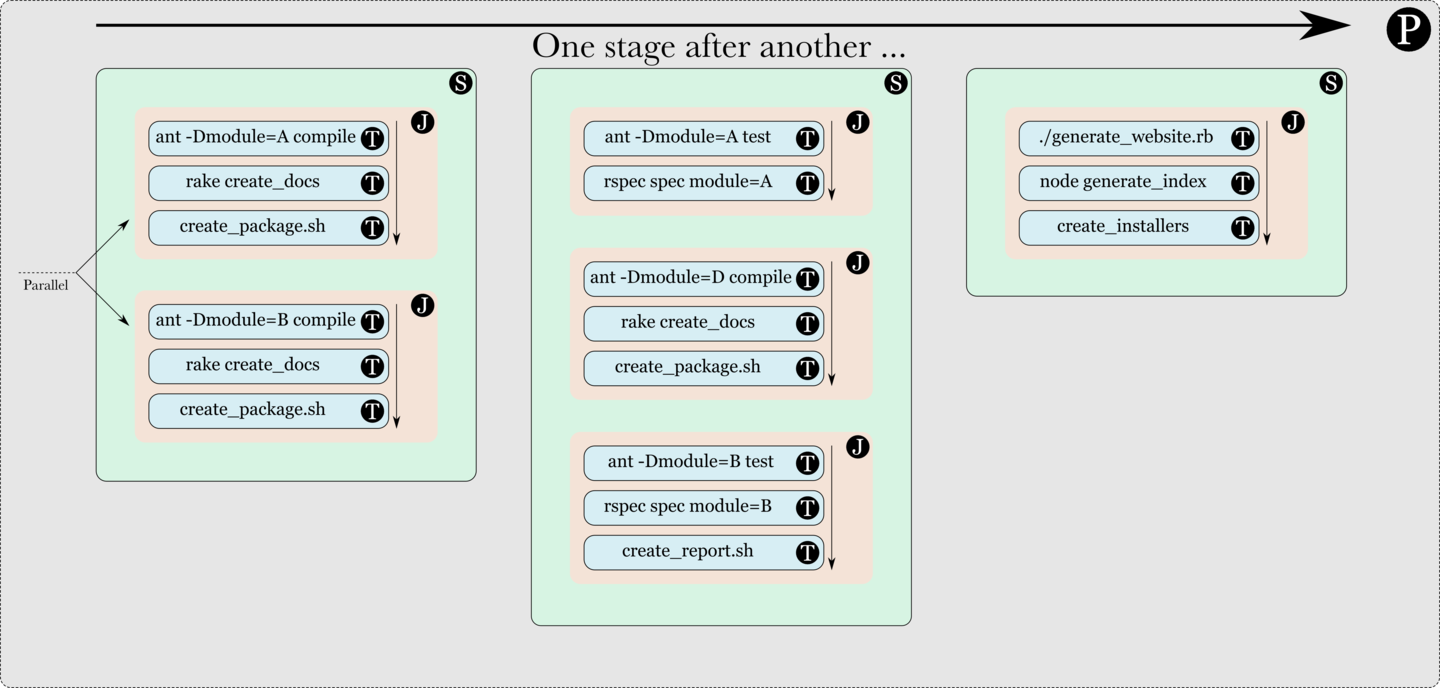
\includegraphics[scale=0.7]{images/pipeline.png}
      \end{center}
      \caption{Schéma du principe d'abstraction de GoCD}
      \label{Pipeline}
    \end{figure}

    Il est dès lors trivial de définir différents \gls{trigger}s (déclencheurs) de comportements pour les Pipelines et les Stages. Si nous avions seulement les deux abstractions Jobs et Stages (comme c'est le cas dans Jenkins par exemple) notre Intégration Continue serait surchagée par les différentes configurations des comportements en fonction des différents contextes.\\

    De plus les Jobs et Stages de GoCD sont des primitives, ce qui inclu qu'ils peuvent, et doivent d'être étendus afin d'obtenir des abstractions de meilleures ordres.\\

    La puissance de cette abstraction réside dans ses éxecutions parallèles et séquentielles:\\

    \begin{enumerate}
      \item de multiples Pipelines peuvent s'exécuter en parallèle,
      \item les multiples Stages d'un Pipeline s'exécutent séquentiellement,
      \item les multiples Jobs d'un Stage s'exécutent en parallèle,
      \item les multiples Tâches dans un Job s'exécutent séquentiellement.\\
    \end{enumerate}

    Ce comportement d'exécution alternée a été délibérement conçu par ThoughtWorks de sorte que nous ayons la possibilité de paralléliser et séquentialiser notre worklow selon ces deux niveaux de granularité.

    \subsubsection{Le concept de First Class au service du pipeline de déploiement de GoCD}
    Le fait que l'on puisse manipuler les abstractions de GoCD comme des fonctions permet de:\\

    \begin{enumerate}
      \item déclencher un Pipeline comme une unité,
      \item faire qu'un Pipeline dépende d'un ou plusieurs autres,
      \item faire traverser des artefacts au travers d'un Pipeline,
      \item avoir le contrôle d'accès au niveau d'un Pipeline,
      \item associer des Pipelines à des environnements,
      \item comparer les changements entre deux instances d'un Pipeline.\\
    \end{enumerate}

    Le pipeline de déploiement peut ainsi dépendre, en entrée, de plusieurs autres Pipelines (fan-in) et de déboucher sur l'exécution de plusieurs autres Pipelines (fan-out) (Voir Figure \ref{VSM}).

    \begin{figure}
      \begin{center}
        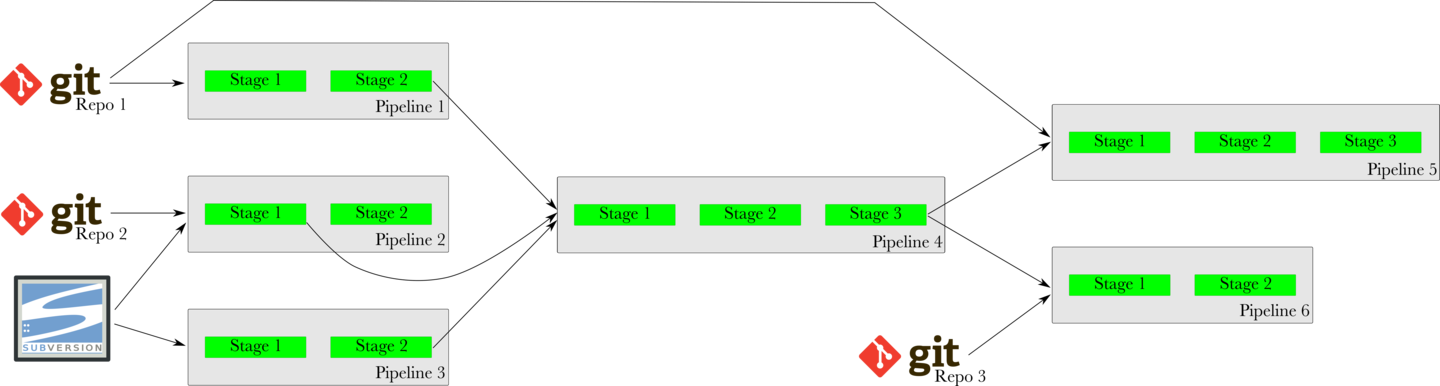
\includegraphics[scale=0.7]{images/VSM.png}
      \end{center}
      \caption{Schéma d'une séquence de Pipelines}
      \label{VSM}
    \end{figure}

    \section{Le référentiel de code source}\label{Repository}
    GoCD intègre parfaitement les divers référentiels de code source. Des agents ont été développés par ThoughtWorks et la communauté de GoCD pour les principaux référentiels de code source (TFS, Git, Github, SVN, Mercurial). De plus GoCD offre la possiblité aux utilisateurs d'utiliser les \gls{webhook}s\footnote{Webhook: Mécanisme servant à notifier des éléments externes à une application web qu'un événement a eu lieu sur celle-ci.} afin de notifier le serveur d'Intégration Continue qu'une modification a été apportée au code source.\\

    Le choix du référentiel de code source dépend essentiellement de la politique interne de versionning de votre entreprise. Dans la suite de ce mémoire nous utiliserons Github comme référentiel de contrôle pour notre plate-forme d'Intégration Continue.

      \subsection{Github}
      Github est un service web d'hébergement et de gestion de code source propriétaire. Cela enfreint un des invariants de notre plate-forme vu précédemment qu'est la qualité open source de notre projet me direz-vous. Certes, cependant Github n'est qu'une surcouche service au gestionnaire de version Git, qui lui, est open-source (Linux - Licence GNU). Pour faire simple Github offre une interface utilisateur et un hébergement dans le cloud à Git.

      Le choix de Github pour cette PIC est simplement dû à une contrainte temporelle. Des alternatives open source sont disponibles sur internet (Gogs, Phabricator, GitBucket) et pourraient être hébergées sur notre serveur d'Intégration Continue. Cepandant Github étant la référence mondiale des référentiels de code source, la plupart des plugins utiles à la réalisation de notre PIC ont déjà été développés par la communauté, ce qui facilitera la mise en place expérimentale de notre serveur d'Intégration Continue.

    \section{Configuration de GoCD}
    La polyvalence d'une plate-forme d'Intégration, outre le choix des outils, réside dans sa configuration. Parfois complexe et fastidieuse la configuration du serveur peut rebuter certains développeurs. Pourtant, une fois maîtrisée et mise en place, les gains apportés par l'Intégration Continue sont non négligeables. Nous allons tenter d'illustrer le pipeline de déploiement d'un projet classique composé d'une unique application.

      \subsection{Configuration générale}
      Après installation du serveur GoCD, pour un usage classique, aucune configuration n'est nécessaire (selon la documentation officielle). GoCD se veut facile d'installation, de configuration et d'utilisation. Cependant je vous conseille fortement de paramétrer la gestion des artefacts ainsi que la sécurité au niveau des accès.

        \subsubsection{La gestion des artefacts}
        Il est fortement conseillé, et ce pour n'importe quel serveur d'Intégration Continue, de créer une partition séparée et extensible sur votre serveur ou dans votre infrastructure pour les artefacts créés. Le dêpot d'artefact peut croître en taille très rapidemment. S'il est situé sur la partition principale de votre système, vous pourriez rencontrer des problèmes de perte de données où de comportement du serveur dans le cas où le disque serait plein.

        \subsubsection{La gestion des accès}
        Le serveur d'Intégration Continue étant au centre de votre développement, doit être régi par une politique d'habilitation afin d'éviter tout problème de disfonctionnement lié à une erreur utilisateur. Les fonctionnalités de gestion des utilisateurs de GoCD vous permettent de contrôler l'accès à votre serveur via un principe d'autorisation basé sur un mécanisme de rôle. Les rôles regroupent un ensemble d'utilisateurs, avec des activités fonctionnelles similaires, et leur accordent un ensemble commun d'habilitations.

      \subsection{Création d'un pipeline de déploiement et de notre premier Stage, le « compile »}
      La première étape à effectuer, dans la configuration d'un processus d'Intégration Continue et de déploiement de GoCD, est de créer un nouveau Pipeline pour notre application. L'interface graphique de GoCD nous propose de faire cela en trois étapes. La première, appelée « Basic Settings », définit le nom de notre Pipeline ainsi que son groupe dans le cas d'un projet multi-applications ou d'une organisation particulière.\\

      La deuxième étape, appelée « Material » permet de définir le point d'entrée de votre Pipeline. Le Material peut-être notre gestionnaire de code source, un package repository (dépôt de binaires) ou encore un autre Pipeline (first class). Dans notre cas nous choisissons de spécifier en point d'entrée notre réferentiel de code source. Pour cela nous sélectionnons le Material « Git », indiquons l'URL du repository Github correspondant à la branche de l'application que nous souhaitons automatiser et définissons la stratégie d'orchestration de notre serveur (Voir la section \ref{ServeurCI}).\\

      La troisième et dernière étape à prendre en compte lors de la mise en place d'un Pipeline est la création de notre tout premier Stage. Cette dernière peut être effectuée manuellement - dans le cadre d'un tout nouveau type de Stage - ou via le biais d'un template prédéfini - rappelons que toutes les configurations de GoCD sont stockées au format XML et donc réutilisables. Ne disposant pas encore d'autre Stage, nous réalisons la configuration de notre Stage de « compile » manuellement. Pour cela nous lui donnons un nom et définissons son type de déclenchement; « On Success » dans le cas d'un trigger automatique basé sur la réussite du Material ou « Manual ». Dans le cas d'une Intégration Continue optimale toutes les actions de cette dernière doivent être automatisées, nous nous tournons donc vers le déclenchement « On Success ». La suite de cette étape de création de Stage est d'initialiser un Job, en lui donnant un nom et une Task, en définissant son type - Ant pour le Java, NAnt pour le .Net, Rake pour le Ruby... - et son répertoire de travail. Dans le cas où aucun type ne correspond à votre besoin vous pouvez directement entrer votre ligne de commande.\\

      Nous venons de construire notre premier pipeline composé d'un Stage de compilation exécuté à chaque commit sur Github.

      \subsection{Les tests}
      A ce stade, notre processus d'Intégration Continue est très sommaire, il effectue exclusivement la compilation de notre code source. L'étape suivante est d'automatiser l'ensemble de nos tests après chaque compilation. Pour cela nous allons mettre en place un nouveau Stage, composé d'un ensemble de Jobs chargés d'exécuter nos différents tests (tests unitaires, tests d'intégration, tests fonctionnels, ...).\\

      Afin d'exécuter nos tests, deux options s'offrent à nous. Nous pouvons utiliser les frameworks propres à chacun et générer des rapports au format XML ou utiliser Gauge, un outil développé par Thoughtworks (à l'origine du développement de GoCD). Bien qu'attrayant, Gauge est encore trop limité au niveau de ses plugins et ne se couple pas avec tous les frameworks de test disponibles. Cependant, GoCD intègre l'agent Gauge Report permettant de visualiser graphiquement les fichiers de sorties des tests aux formats XML. L'exécution des tests sera donc automatisé par ligne de commande et reporté graphiquement via l'interface du site web (Voir la figure \ref{GoCDReportTest}).\\

      Nous définissons donc un nouveau Stage qui sera composé d'autant de Jobs que de types de tests effectués. Chaque Job pourra contenir une ou plusieurs tasks en fonction de votre découpage. Le déclencheur de ce Stage de test sera le succès du Stage de compilation.

      \begin{figure}
        \begin{center}
          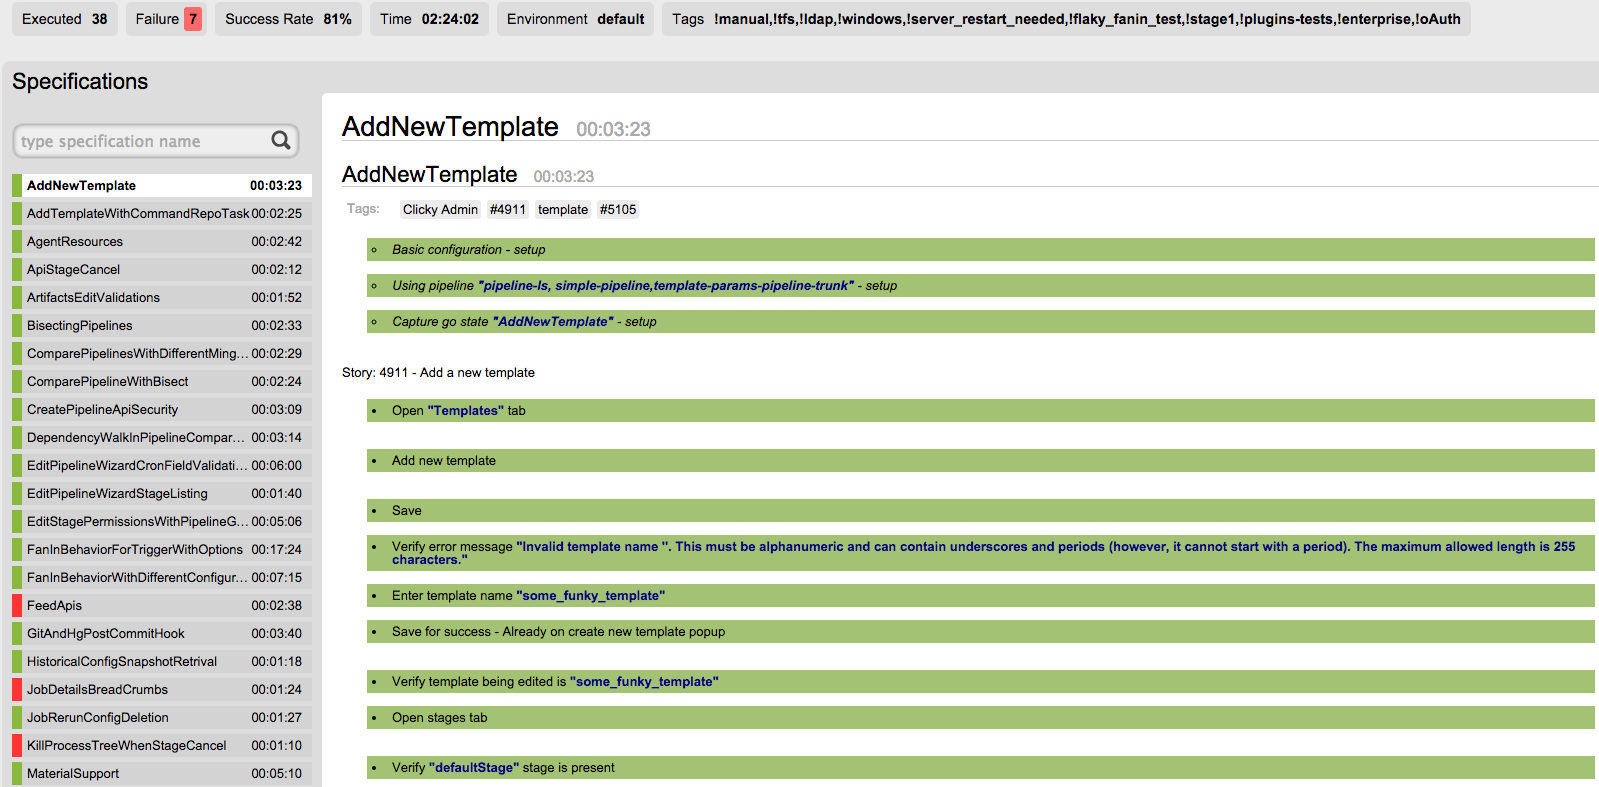
\includegraphics[scale=0.15]{images/GoCDReportTest.png}
        \end{center}
        \caption{Visualisation d'un rapport de test dans GoCD}
        \label{GoCDReportTest}
      \end{figure}

      \subsection{L'inspection du code}
      L'inspection statique du code source est une étape majeure dans l'assurance qualité de l'Intégration Continue. Déjà présente et configurée au sein des pipelines de déploiement des projets AXA via l'outil SonarQube, nous allons l'intégrer au sein de notre PIC. Reprenons notre configuration illustrative d'un Pipeline de déploiement classique; il contient actuellement le Stage de compilation et le Stage de test. L'inspection de code source se situe en amont de la compilation. Nous allons donc créer un nouveau Stage qui prendra en Material le gestionnaire de code source et qui sera le point d'entrée du Stage de compilation. Ce Stage sera chargé d'exécuter SonarQube et d'enregister le rapport au format HTML pour qu'il puisse être affiché par un agent de GoCD (Voir la figure \ref{GoCDSonar}).\\

      \begin{figure}
        \begin{center}
          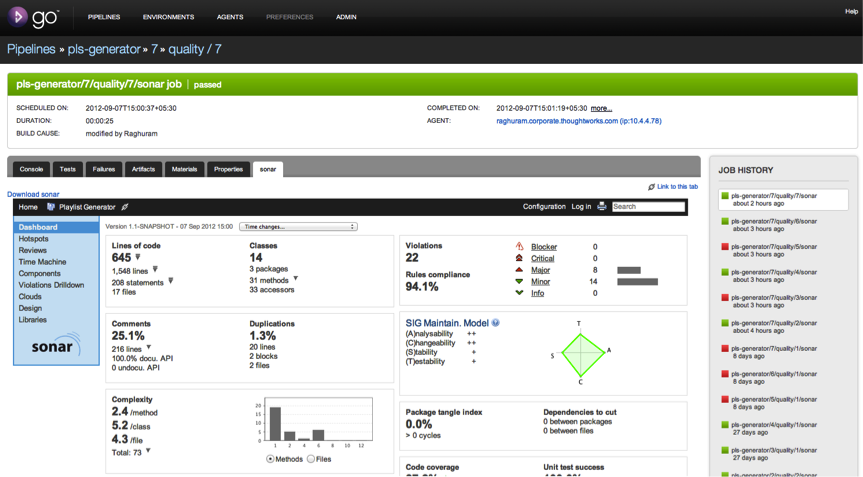
\includegraphics[scale=0.7]{images/GoCDSonar.png}
        \end{center}
        \caption{Visualisation d'un rapport d'analyse statique de code dans GoCD}
        \label{GoCDSonar}
      \end{figure}

      % \subsection{La documentation}

      \subsection{Le packaging}
      L'ultime étape avant celle du déploiement est le packaging de notre solution. Elle consiste à rassembler l'ensemble des dépendances d'une application au sein d'un même package - qu'il soit un zip, un conteneur, un exécutable (.exe), un msi (Microsoft Installer), un war (Wep application Archive)... - afin de faciliter le déploiement sur serveur. Le type de package attendu dépendra essentiellement du langage de l'application, de votre infrastructure et de la politique de déploiement de votre compagnie. Chez AXA, les applications Java sont packagées en war, les application .NET en msi et les applications Javascript en zip. Les conteneurs ne sont pas encore utilisés faute de non compatibilité de nos serveurs.\\

      Dans le cadre de notre solution, où nous désirons déployer dans le Cloud, la compatibilité des serveurs ne nous pose aucun problème. Les fournisseurs de Cloud assurent la disponibilité des dernières versions des systèmes d'exploitation. Nous pouvons donc utiliser les conteneurs comme type de package pour nos applications. Nous devons créer un nouveau Stage, responsable du packaging, qui sera chargé de la création et de la configuration de notre container Docker. Cet artefact sera le Material du Stage de déploiement.

      \subsection{Le déploiement}
      La dernière étape de notre Pipeline est le déploiement de notre package dans le Cloud. De part sa complexité nous n'allons pas nous attarder sur la mise en place de ce Stage. Vous devez juste avoir en tête qu'il sera responsable du provisionning du serveur, de la distribution de l'artefact de build et de son installation.

      \subsection{Architecture et fonctionnement de la PIC}
      A ce stade du mémoire, notre plate-forme d'Intégration Continue est hébergée sur un serveur interne physique. Notre référentiel de code source, hébergé par Github, repose sur l'approche du « post commit hook » (Voir la section~\ref{ServeurCI}). Lorsqu'un développeur pousse son code sur Github, le gestionnaire de code source notifie le serveur d'Intégration Continue qui déclenche l'exécution de son pipeline de déploiement. Les utilisateurs peuvent visualiser l'avancement de leur Intégration Continue sur l'interface web de GoCD (Voir Figure \ref{PICv1}).\\

      L'installation, la configuration et la maintenance de notre PIC est, pour l'heure, entièrement manuelle.\\

      \begin{figure}
        \begin{center}
          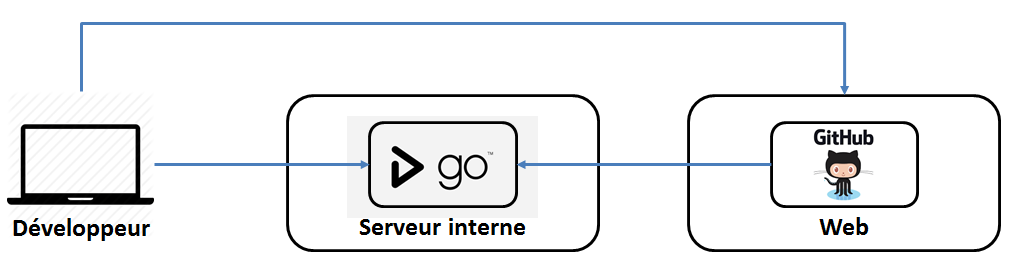
\includegraphics[scale=0.5]{images/PICv1.png}
        \end{center}
        \caption{Schéma de la première version de notre PIC - Standard}
        \label{PICv1}
      \end{figure}

    \section{Migration de la plate-forme d'Intégration Continue dans le Cloud public}
    Le Cloud Computing a récemment émergé comme un nouveau paradigme pour l'hébergement et la prestation de services sur Internet. Il est attrayant pour les entreprises car il élimine la nécessité pour les utilisateurs de planifier à l'avance l'approvisionnement des serveurs et leurs permet de commencer avec de petites ressources pour les augmenter en fonction de la demande. En dépit du fait que le Cloud Computing offre d'énormes possibilités pour l'industrie informatique, le développement de ses technologies et de ses utilisations est actuellement à ses débuts.

      \subsection{La valeur ajoutée}
        \subsubsection{L'Agilité}
        Le Cloud Computing accélère et simplifie le provisionnement et la réallocation des ressources de l'infrastructure informatique. Selon nos besoins nous pourrons mettre en oeuvre de nouvelles applications, modifier la structure de l'infrastructure, ou augmenter/réduire l'utilisation de nos ressources afin d'améliorer notre Intégration Continue. De plus, notre serveur d'Intégration Continue sera accessible hors du domaine réseau d'AXA, offrant ainsi une plus grande mobilité aux équipes de développement.

        \subsubsection{La scalabilité}
        La puissance de traitement des charges de travail de notre serveur d'Intégration Continue fluctue en fonction du temps, des actions et des projets. Une plus grande puissance est requise lors de l'exécution d'un pipeline de déploiement que lors d'une simple visualisation de l'état de nos différentes builds par exemple. C'est ce que l'on appelle la scalabilité de l'infrastructure. L'infrastructure de type Cloud adapte la capacité et le nombre de serveurs aux besoins réels tandis que les infrastructures traditionnelles sont conçues pour répondre aux besoins lors des périodes d'utilisation intensives.

        \subsubsection{Les coûts}
        Les ressources Cloud fonctionnent sur le principe du service à la demande. Les entreprises ne paient que ce qu'elles consomment. Les besoins en ressource d'une PIC varient en fonction du cycle de développement des projets présents. Couplée au principe de la scalabilité, la migration de notre serveur d'Intégration Continue dans le Cloud permet de reduire le budget assigné à l'infrastructure.

        \subsubsection{La fiabilité et les sinistres}
        Les fournisseurs de Cloud intègrent à leur plate-forme des mécanismes de migration dynamique, de migration du stockage, de tolérance aux pannes (haute disponibilité) et de planification des ressources distribuées. Ces fonctionnalités accroissent le temps de disponibilité et accélèrent les procédures de restauration. En cas de sinistre, des mécanismes de réplication automatique sont mises en place, offrant une disponibilité quasi illimitée à notre serveur d'intégration.

        \subsubsection{L'« Infrascture As Code » au service de la qualité et de la cohérence}
        De nombreuses équipes informatiques comptent encore sur les configurations manuelles, des scripts, des images ou des outils obsolètes pour gérer l'infrastructure, ce qui entraîne des erreurs et des déploiements lents. Les organisations qui cherchent à améliorer la qualité et la cohérence de leurs infrastructures traitent ces dernières comme des applications; ils codent leurs infrastructures. Ce code pourra dès lors être intégré dans un processus d'Intégration Continue ce qui permet de tester, normaliser et garantir l'unicité du système afin d'éviter les imprévus.\\

        Chaque fournisseur de Cloud dispose de ses propres mécanismes et outils pour coder votre infrastructure, ce qui peut être déroutant si votre système d'information s'appuie sur plusieurs fournisseurs de Cloud. Pour cela des solutions tierces ont vu le jour (Ansible, Chef, Puppet) et proposent des « templates » afin de provisionner vos instances sur tous types de Cloud.

      \subsection{Les préjugés}
        \subsubsection{La sécurité}
        La sécurité est un axe majeur dans le débat sur le Cloud public. Les données, propres à l'entreprise, sont ainsi exposées sur internet et nécessitent un cadre d'utilisation strict. La sécurité au niveau de la couche d'accès au réseau et de la couche applicative du Cloud (selon le protocole TPC/IP) est généralement controlée par les fournisseurs de Cloud eux-mêmes. Ces derniers assurent entre autre les communications entrantes et sortantes autorisées par les instances (pare-feux), la protection des données (en les stockant dans des data centers hautement sécurisés), le respect des exigences en matière de conformité, la mise en place de politiques d'accès utilisateurs (création de groupes de sécurité) et applicatives (création de clés d'accès) ...

        % \subsubsection{Les performances}

        \subsubsection{La perte de contrôle}
        Les départements informatiques internes sont habitués à gérer l'intégralité des serveurs de leur entreprise et peuvent avoir des réticences à déléguer certains de leurs pouvoirs à un fournisseur de Cloud externe (Amazon Web Services, Azure, Google Cloud). Cette réticence peut être motivée par des doutes légitimes sur la capacité intrinsèque du Cloud et du fournisseur ou par une peur de la perte de leur emploi. En réalité, le Cloud Computing public propose une capacité généralement supérieure à celle dont dispose la plupart des entreprises. Les infrastructures et services proposés par les fournisseurs sont de plus en plus poussés nécessitant une connaissance profonde des plate-formes de Cloud et l'émergence au sein de l'entreprise d'expert du Cloud public.

      \subsection{Le choix du fournisseur de Cloud}
      Le choix du fournisseur de Cloud est un problème épineux. De nombreux critères entrent en compte tels que le temps de disponibilité, l'infrastructure, la gestion des changements, la sécurité, la surveillance, la sauvegarde et l'archivage, l'intéropérabilité, la migration, l'évolutivité, la continuité d'activité, la visibilité, le service, le support, les coûts...\\

      De même que pour le référentiel de code source, le choix du fournisseur de Cloud dépendra essentiellement de la politique Cloud de votre entreprise. Dans notre cas nous utiliserons la plate-forme Amazon Web Services (\gls{AWS}) pour héberger les différentes instances composant notre PIC.

      \subsection{La migration de GoCD dans AWS}
      Dans un premier temps nous allons déployer notre serveur d'Intégration Continue sur une machine virtuelle Linux dans le Cloud d'Amazon. Pour des raisons de sécurité seuls les ports SSH et de GoCD seront ouverts à une population restreinte d'adresse IP (utilisateurs et Github). Les différents utilisateurs pourront ainsi accéder à la plate-forme d'Intégration Continue via leur navigateur web.\\

      Les machines virtuelles du Cloud, une fois codées, sont amenées à avoir des cycles de vie et de renouvellement courts. Afin de pérenniser les données nous devons stocker l'intégralité de leurs ressources dans un environnement de stockage durable.

        \subsubsection{A propos d'AWS}
        Amazon Web Services, proposé par Amazon, est un des leaders du Cloud public. Il offre un catalogue riche de services répondant aux besoins de provisionning, de stockage, de base de données, de réseaux, de sécurité, d'analytiques, d'\gls{IoT}\footnote{IoT (Internet Of Things): l'internet des objets}... Nous n'étudierons pas chacun de ses services - Amazon propose plus de 700 heures de formation - mais nous allons nous intéresser à deux services en particulier: Amazon Elastic Compute Cloud (\gls{EC2}) et Amazon Simple Storage Service (\gls{S3}).\\

        Amazon Web Services propose pour tous ses services une interface graphique en ligne ainsi qu'une \gls{API}\footnote{Application Programming Interface (API): ensemble normalisé de classes, methodes ou fonctions servant de façade par laquelle une application offre ses services aux autre applications.} afin de pouvoir intéragir avec eux au travers d'outils tiers.\\

        \begin {boxedminipage} {11cm}
          Les services étudiés sont propres à la plate-forme AWS, cependant les autres fournisseurs de Cloud proposent des services similaires dans leur fonctionnement. Nous nous intéressons ici au concept de ces services et non pas aux services eux-mêmes.
        \end {boxedminipage}\\

          \paragraph{EC2, l'hébergeur de serveur virtuel}
          Amazon Elastic Compute Cloud (Amazon EC2) est un service Web qui fournit une capacité de calcul redimensionnable dans le cloud. Destiné aux développeurs, il est conçu pour faciliter l'accès aux ressources de cloud computing à l'échelle du Web. Il fonctionne sur le principe d'Instance (machine virtuelle) reposant sur le mécanisme de « Platform As A Service » (PAAS) (Voir la section~\ref{CloudComputing}) et qui est donc entièrement configurables.

          \paragraph{S3, le service de stockage}
          Amazon Simple Storage Service (Amazon S3) offre aux développeurs et aux équipes informatiques un espace de stockage dans le cloud sécurisé, durable et hautement évolutif. Les données sont organisées en Buckets - propres à chaque compte Amazon Web Services - et identifiées par une clé unique attribuée par l'utilisateur (principe de la clé/valeur).

        \subsubsection{Coder le provisionning des instances}
        Le Cloud Computing insiste fortement sur la notion d'« Infrastructure As Code ». Lorsque notre infrastructure est décentralisée dans le Cloud et que nous devons faire des déploiements fréquents de services sur des serveurs globalement identiques, l'automatisation et la maintenance de cette dernière au travers du code se révèle primordiale. Les environnements peuvent ainsi être testés, mis sous contrôle de version, réutilisés et partagés.\\

        Notre solution se voulant être agnostique du fournisseur de Cloud nous utiliserons un outil de provisionning indépendant. Ce dernier nous permet d'utiliser des recettes, playbooks, modèles ou quelle que soit la terminologie employée afin de simplifier l'automatisation et l'orchestration de nos environnements.

          \paragraph{Le choix de l'outil}
          Il y a plusieurs considérations à garder à l'esprit lors du choix d'un outil de provisionning. Le première est le modèle de l'outil; certains s'appuient sur un modèle de maître-esclave qui utilise un point de contrôle centralisé et communique avec les machines distribuées, d'autre préfèrent fonctionner à un niveau plus local. Une autre considération à prendre en compte est la composition de votre environnement, certains outils ne supportent pas l'intégralité des systèmes d'exploitation.

          \paragraph{Ansible un bon compromis}\label{Ansible}
          Ansible est un outil open source utilisé pour déployer des applications sur des noeuds distants (le Cloud par exemple) et provisionner les serveurs de façon reproductible. Il offre un cadre commun pour pousser les applications multi-niveaux et des artefacts d'appliction à l'aide d'une configuration de modèle push, mais nous pouvons aussi le configurer en tant que maître-esclave. Ansible est construit sur le principe de Playbook qui englobe les configurations du serveur, le deploiement et l'orchestration.\\

          Si nous voulons une prise en main rapide et facile et que nous ne voulons pas installer des agents sur les noeuds distants ou les serveurs gérés, Ansible est un très bon compromis. Il se concentre sur le fait d'être rationalisé et rapide. Il met à la disposition de ses utilisateurs un dépôt (Ansible Galaxy), alimenté par la communauté, afin de proposer des Playbooks pré-configurés.\\

          De plus, Ansible Tower un soft cette fois-ci payant, permet de contrôler et monitorer l'ensemble de ses déploiements.

          \paragraph{Développement de notre Playbook}
          Le réflexe à avoir, lorsque que l'on travaille avec une technologie disposant d'un dépôt open source, est de chercher si la communauté n'a pas déjà travaillé et mis à disposition un artefact répondant à nos besoins. Dans notre cas, en cherchant sur Ansible Galaxy nous tombons sur plusieurs Playbooks incluant le téléchargement, l'installation et la configuration de GoCD sur un serveur. Proposant des fonctionnalités analogues nous nous dirigeons vers le projet le mieux noté et disposant de la plus grande communauté.\\

          Mais le déploiement de GoCD ne correspond qu'à un rôle dans le Playbook de provisionning de notre plate-forme d'Intégration Continue dans le Cloud. En effet le rôle GoCD installe l'outil sur un serveur cible, or nous n'avons pas pour l'instant automatisé le provisionning d'une instance dans AWS. Notre Playbook doit ainsi définir un rôle AWS, en amont du rôle GoCD, afin de créer et configurer automatiquement l'instance EC2. Pour cela nous suivons le schéma précédent et trouvons sur Ansible Galaxy un projet de provisionning dans le Cloud d'Amazon. Nous avons dès lors automatisé l'intégralité de la chaîne de déploiement d'une instance GoCD dans le Cloud.\\

          \begin {boxedminipage} {11cm}
            Le code chargé du provisionning des instances varie en fonction des divers systèmes d'exploitation. Dans le cadre de notre projet open source nous soumettons l'hypothèse que l'environnement cible de notre plate-forme d'Intégration Continue est une des multiples distributions Linux.
          \end {boxedminipage}\\

        \subsubsection{Externaliser les données de GoCD dans un service de stockage}
        Externaliser les données de GoCD dans S3 s'avère obligatoire si nous voulons assurer la pérennité de ces dernières. GoCD s'appuie sur deux types de données; les données de configuration et les artefacts créés par les Pipelines.

          \paragraph{Les données de configuration} L'intégralité des données de configuration liées à GoCD (configuration du serveur, des Pipelines, des Tâches, des Jobs...) sont présentées sous la forme de fichier XML. Globalement leur externalisation est assez simple, il suffit de renseigner dans le fichier de configuration du serveur (Config.xml) leur localisation dans le bucket S3 et le tour est joué. Cependant cette approche ne peut être appliquée au Config.xml car comment indiquer au serveur la localisation de son propre fichier de configuration ? Pour pallier cette complexité cyclique nous devons créer une copie du fichier externalisé dans S3 et le coller au niveau de la racine de GoCD dans l'Instance. Bien évidemment cette étape est à automiser lors du déploiement du serveur d'Intégration Continue avec Ansible.

          \paragraph{Les artefacts} L'exécution d'un Pipeline peut amener à la création d'un ou plusieurs artefacts réutilisables par d'autres Pipelines. Lors de l'exécution de ces autres Pipelines, il peut s'avérer inutile de relancer le Pipeline responsable de la production de l'artefact si ce dernier n'a subi aucune modification. GoCD propose donc d'archiver ces artefacts. L'externalisation de ces derniers dans S3 se fait au niveau de son fichier Config.xml (ou via son interface utilisateur) (Voir Figure \ref{ArtifactsDir}).\\

          \begin{figure}
            \begin{center}
              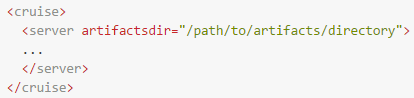
\includegraphics[scale=0.7]{images/ArtifactsDir.png}
            \end{center}
            \caption{Externalisation des artefacts dans GoCD}
            \label{ArtifactsDir}
          \end{figure}

          \paragraph{Configurer l'externalisation des données dans notre Playbook} Dans notre objectif de mettre en place une PIC intégralement « codée » nous devons automatiser cette externalisation via notre Playbook. Dans notre rôle GoCD, nous devons ajouter deux nouvelles tâches qui auront pour but de modifier le fichier de configuration de notre serveur d'Intégration Continue afin qu'il prenne en compte l'externalisation des données.

        \subsection{Architecture et fonctionnement de la PIC}
        Avec cette première version Cloud de notre plate-forme d'Intégration Continue notre serveur GoCD est hébergé durablement dans une Instance EC2 du le Cloud d'Amazon Web Services. L'intégralité de ces données (configurations et artefacts) est stockée dans un Bucket S3 afin de pérenniser ces ressources. La création de l'Instance, le déploiement de GoCD et sa configuration sont codés et gérés par Ansible, notre outil de provisionning.\\

        Comme avec la version locale, les développeurs déclenchent l'exécution d'un pipeline de déploiement lors d'un push sur Github. Les utilisateurs peuvent directement intéragir avec GoCD par le biais de son interface web (Voir Figure \ref{PICv2}).\\

        \begin{figure}
          \begin{center}
            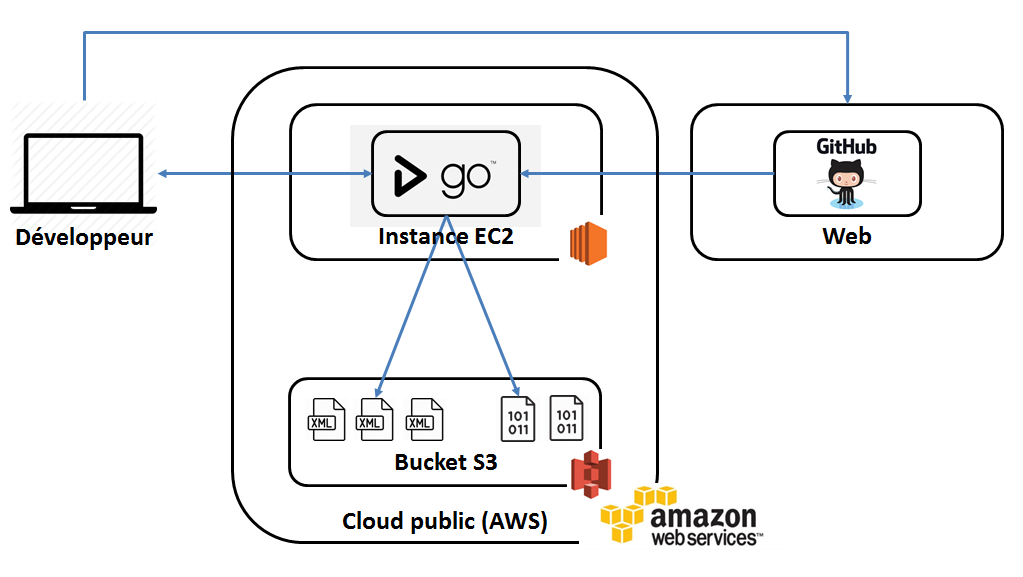
\includegraphics[scale=0.5]{images/PICv2.png}
          \end{center}
          \caption{Schéma de la seconde version de notre PIC - Cloud I}
          \label{PICv2}
        \end{figure}

      \section{Amélioration de la plate-forme d'Intégration Continue en se basant sur le principe du Cloud des instances à la demande}
      Le pilier du Cloud « Infrascture As Code », couplé à un démarrage rapide des instances garanti par les fournisseurs de Cloud, apporte une évolution dans la gestion des serveurs au sein des entreprises; les serveurs sont vus comme des consommables que l'on crée et détruit en fonction des besoins. Par exemple, les instances hébergeant les applications internes d'une entreprise (uniquement utilisées par ses collaborateurs) peuvent être détruites en fin de soirée et relancées au petit matin, du fait de leur non-utilisation la nuit. Cette nouvelle méthodologie permet de réduire les coûts d'infrastructure tout en garantissant un environnement propre et homogène à nos applications.\\

      Selon les phases d'avancement de notre projet le code source évolue différemment - une évolution forte lors de sa phase de développement et faible lors de sa maintenance applicative - ce qui entraine une utilisation non-homogène de notre PIC. De plus, si notre équipe de développement est exclusivement composée de développeurs travaillant selon le même fuseau horaire, la sollicitation de notre serveur d'Intégration Continue lors de sa phase de développement n'est pas non plus également répartie, avec une demande forte en journée et quasi nulle la nuit. Le principe d'instance à la demande peut tout à fait être utilisé dans le cas de notre plate-forme.\\

        \subsection{Ansible notre provisionneur d'instance}
        Dans la section précedente nous avons vu comment Ansible (Voir la section~\ref{Ansible}), un outil de provisionning, pouvait automatiser la création et la configuration de notre serveur d'Intégration Continue dans le Cloud. Nous allons réutiliser ce procédé pour nos instances à la demande.\\

        La solution d'instance à la demande transforme la précedente architecture de notre PIC (Voir Figure \ref{PICv2}). Notre serveur d'Intégration Continue ne sera plus composé d'un serveur d'Intégration Continue mais d'Ansible, notre provisionneur d'instance, qui sera chargé de créer et détruire les instances éphémères qui hébergeront GoCD. Nous aurons ainsi une instance Ansible qui gérera une multitude de serveurs d'Intégration.

        \subsection{Le cycle de vie d'une instance hébergeant notre serveur d'Intégration Continue}
        Maintenant que nous avons défini nos instances GoCD comme étant à la demande et éphémères, se pose la question du cyle de vie de ces instances; quand Ansible doit-il créer et détruire un serveur GoCD?\\

          \subsubsection{Une instance à chaque commit sur le serveur de contrôle de code source}
          La première approche naïve, et la plus simple, est de demander à Ansible de provisioner un serveur d'Intégration Continue à chaque fois qu'un développeur pousse son code dans le référentiel de code source et de tuer l'instance à la fin du pipeline de déploiement. Simple, cette solution n'est cependant pas optimale. Rappelons-nous que certaines équipes de développement effectuent plus de cinquante déploiements par jour, soit plus d'un déploiement toutes les dix minutes. Multiplié par le nombre de projets gérés par notre PIC, nous arrivons à un nombre de provisionnement considérable géré par une unique instance Ansible, impactant ainsi ses performances.

          \subsubsection{Une instance par cycle de développement}
          La seconde approche pour gérer le cycle de vie de nos instances GoCD est de considérer les cycles de notre application et d'allouer un serveur d'Intégration Continue à chaque phase de développement. Notre serveur GoCD serait ainsi disponible durant toute la période de développement et tué lors des périodes de non activité. Le principe d'instance à la demande est respecté mais très peu utilisé.

          \subsubsection{Une instance par jour}
          Dans le cas ou l'intégralité de l'équipe de développement travaille selon le même fuseau horaire nous pouvons définir une politique d'instance journalière lors des cycles de développement. L'instance GoCD serait provisionnée le matin lors du premier commit et détruite chaque soir.

          \subsubsection{Une instance adaptée}
          La dernière approche, et la plus optimisée, s'adapte au besoin de l'équipe de développement en détruisant l'instance GoCD après une période d'inactivité de l'ordre de l'heure (définie par l'équipe). Si lors d'un commit une instance est présente dans le cloud, elle est utilisée sinon Ansible en déploie une nouvelle. Le principe de l'instance à la demande est ainsi optimisé et garantit une infrasctructure à moindre coût.

        \subsection{Automatiser l'intelligence de notre infrastructure}
        Ansible, quoique très puissant, ne peut gérer le cycle de vie de nos instances GoCD. Il ne possède pas de mécanisme d'écoute d'évènement. Il nous faut donc ajouter un \gls{middleware}\footnote{Middleware: logiciel tiers créant un réseau d'échange entre différentes applications.} entre notre référentiel de code source et notre outil de provisionning afin que ces derniers puissent communiquer.\\


          \subsubsection{Un middleware d'écoute}
          Nous avons vu précédemment que notre référentiel de code source communiquait avec notre serveur d'Intégration Continue via des agents ou via le mécanisme de Webhooks (Voir la section~\ref{Repository}). Ansible, actuellement la seule entité présente de façon durable dans notre PIC, ne possède aucune fonctionnalité citées ci-dessus. La communication entre Github et Ansible est donc impossible. Nous devons ainsi ajouter un outil d'écoute capable de lancer automatiquement et intelligemment des scripts.\\

          La première approche, la plus intuitive mais la plus coûteuse et la moins maintenable, serait de développer un petit outil interne. Ca a été l'approche effectuée par Github pour sa propre plate-forme d'Intégration Continue. Cependant, devant l'engouement et le succès de son outil, Github a fait évoluer cet outil comme une des pierres angulaires de sa PIC et a décidé de publier son outil afin d'en faire un standard, Hubot.

          \subsubsection{Hubot le robot de votre entreprise}\label{Hubot}
          Hubot est un outil d'automatisation de script (CoffeeScript) qui se synchronise avec des services de chat tel que Slack ou HipChat (nous verrons l'utilité de cette fonctionnalité ultérieurement). Initialement développé par Github, Hubot est aujourd'hui un projet open source. Standardisés, les scripts sont partageables et disponibles sur Github.\\

          Dans un premier temps notre robot Hubot doit être capable de recevoir des notifications de Github (ou de tout autre référentiel de code source) et d'exécuter un script Ansible en fonction du cycle de vie de notre serveur d'Intégration Continue. Github et la communauté, très active, proposent un script de notification de Github via les Webhooks ainsi qu'un script exécutant les Playbooks d'Ansible. De notre côté nous devons développer un troisième script qui, appelé par le script de Github, exécutera le script d'Ansible en fonction de la gestion du cycle de vie de l'instance de GoCD vu précédemment (Voir figure \ref{HubotScripts1}).\\

          \begin{figure}
            \begin{center}
              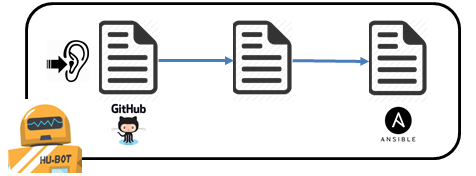
\includegraphics[scale=0.7]{images/HubotScripts1.png}
            \end{center}
            \caption{Hubot - Gestion des notifications de Github}
            \label{HubotScripts1}
          \end{figure}

      \subsection{La chatroom, le point d'entrée de notre plate-forme d'Intégration Continue}
      Un des bénéfices primaires de l'Intégration Continue est d'améliorer la visibilité du projet en fournissant des informations en temps réel sur l'état des builds ainsi que des rapports sur la qualité du code source. En faisant évoluer notre serveur GoCD en instance à la demande nous perdons l'aspect permanent de cette visibilité - si l'instance GoCD n'est pas déployée et active, nos utilisateurs ne disposent d'aucun point d'entrée sur notre PIC. Nous devons ainsi mettre à la disposition des utilisateurs de l'Intégration Continue une interface permanente afin qu'ils puissent intéragir avec notre serveur.\\

      Cette nouvelle interface doit respecter quatre grands principes si nous voulons qu'elle ajoute de la valeur à notre plate-forme d'Intégration Continue:\\

      \begin{itemize}
        \item la permanence: pour répondre à la contrainte du serveur GoCD à la demande,
        \item l'omniscience: toutes les informations sur l'Intégration Continue doivent y figurer,
        \item l'intérêt: l'interface doit avoir un intérêt autre que celui de GoCD,
        \item l'évolutivité: afin d'y intégrer de nouvelles fonctionnalités.\\
      \end{itemize}

        \subsubsection{Les principes fondamentaux de notre point d'entrée}
          \paragraph{La permanence} Nous avons déjà évoqué précédemment la qualité de permanence - indispensable - du point d'entrée de notre PIC. Les informations créées et stockées sur notre serveur d'Intégration Continue doivent être disponibles à tout moment et récupérées facilement. Notre interface devra donc être déployée sur un serveur pérenne, issu de nos serveurs privés ou du Cloud, accessible par tous et de partout.
          Dans notre cas, le point d'entrée sera installé sur notre serveur hébergeant Ansible et Hubot mais il pourra tout aussi bien être installé sur un serveur distant ou fonctionner en mode SaaS (Voir l'annexe \ref{CloudComputingAnnexe}).

          \paragraph{L'omniscience} Notre point d'entrée, et notre unique correspondant avec notre serveur, doit être capable de restituer l'intégralité des informations produites par la PIC. Cette restitution doit être claire, lisible et graphique.
          GoCD stocke la totalité de ses informations sous forme de fichier XML. Notre interface devra être capable d'interpréter le XML et de le retranscrire graphiquement.

          \paragraph{L'intérêt} Notre interface, outre le fait qu'elle implémente des services analogues à ceux proposés par GoCD, doit proposer de nouvelles fonctionnalités ayant pour but d'améliorer l'Intégration Continue.
          Un des points faibles des plate-formes d'Intégration Continue est la notion de communication - qu'elle soit entre le serveur et les utilisateurs ou entre les utilisateurs eux-mêmes. La PIC induit à une communication asynchrone souvent mal gérée. La communication entre les acteurs d'un même projet est très importante. L'intérêt de notre point d'entrée serait de fournir un mécanisme de communication asynchrone et tracée car les conversations que l'on a autour du code sont aussi importantes que le code lui-même. L'idée serait d'avoir au même endroit que notre produit fini (le code) la « recette » qui nous a permis d'y arriver.

          \paragraph{L'évolutivité} L'Intégration Continue est un concept jeune qui ne cesse d'évoluer. Notre interface devra être capable d'intégrer et de centraliser les fonctionnalités qui seront présentes dans les futures implémentations des plate-formes d'Intégration Continue.
          Devant l'inconnue de ces futures fonctionnalités, le meilleur outil que nous pouvons utiliser pour les intégrer reste la ligne de commande. La ligne de commande permet aux utilisateurs d'un service informatique d'exécuter une commande prédéfinie, accompagnée de ces arguments; l'évolutivité est ainsi infinie.

        \subsubsection{Le choix de notre point d'entrée: la chatroom}
        Cette section va être consacrée au choix de l'outil que nous allons utiliser comme point d'entrée de notre PIC. Commençons par faire un petit récapitulatif des fonctionnalités que doit proposer cet outil:\\

        \begin{itemize}
          \item un mécanisme de réprésentation des informations de l'Intégration Continue,
          \item un mécanisme de ligne de commande pour intéragir avec notre serveur,
          \item un mécanisme de communication asynchrone.\\
        \end{itemize}

        Maintenant rappelons nous qu'Hubot a été conçu par les équipes de Github pour s'intégrer à des plate-formes de communication collaborative telles que Slack et HipChat (Voir la section \ref{Hubot}). En étudiant ces outils nous remarquons qu'ils remplissent les trois fonctionnalités essentielles de notre point d'entrée; de part leur nature ils fournissent une communication asynchrone et disposent d'une interface graphique pour la représentation des informations ainsi qu'une zone de saisie de texte pour le mécanisme de ligne de commande (Voir figure {\ref{Slack}}). De plus, le principe des plate-formes de travail collaboratif est déjà fortement présent au sein des équipes, l'utilisation d'un tel outil n'est ainsi pas déconcertant pour les collaborateurs. Nous allons donc nous appuyer sur cet outil pour notre point d'entrée.\\

        \begin{figure}
          \begin{center}
            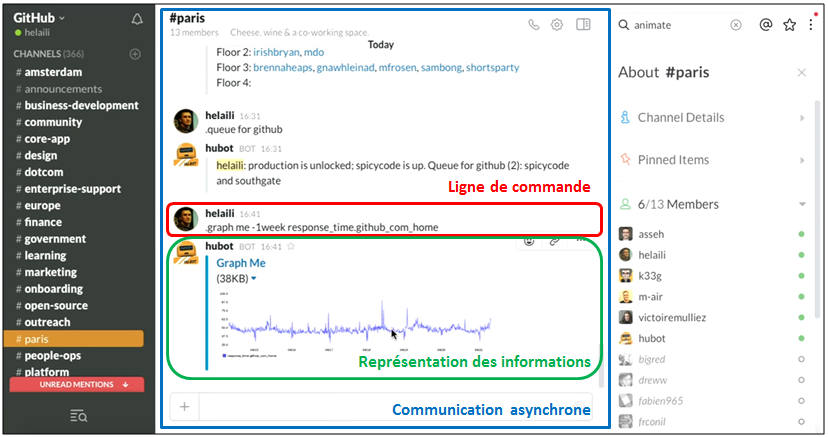
\includegraphics[scale=0.5]{images/Slack.png}
          \end{center}
          \caption{Slack - Example d'une chatroom au sein des équipes de travail à Github}
          \label{Slack}
        \end{figure}

        Les plate-formes de communication collaborative, très à la mode ces dernières années, sont fortements présentes sur le marché (Slack, HipChat, Mattermost, ...). Le choix de telle ou telle plate-forme dépendra essentiellement de votre entreprise, mais toutes offrent globalement les mêmes services. Il vous faudra juste vérifier la disponibilité d'un adaptateur Hubot pour que ce dernier puisse communiquer avec. Dans le cas contraire libre à vous de développer et de soumettre votre plugin à la communauté. Dans notre cas d'une plate-forme d'Intégration Continue open-source nous allons nous tourner vers Mattermost, une alternative open source à Slack.

        \subsubsection{Les communications}
          \paragraph{Une communication asynchrone entre les collaborateurs}
          La communication asynchrone est souvent négligée dans les entreprises. Sans traçabilité, archivage et partage des conversations de nombreuses décisions sont remises en cause ou non appliquées. De plus avec l'internalisation des organisations, des équipes de travail se trouvent distribuées à travers la planète, sur des fuseaux horaires différents. Il faut qu'ils puissent travailler ensemble sans se voir, sans appels vocaux ou visuels. Il faut donc instaurer un mode de fonctionnement qui leur permet de collaborer sans perte de temps et d'efficacité. La communication asynchrone répond à ces deux problématiques.

          \paragraph{Une communication par ligne de commande entre les collaborateurs et Hubot}
          Outre la communication avec les autres collaborateurs, Mattermost permet de communiquer avec Hubot, notre robot d'Intégration Continue. Ce lien nous permet d'avoir un point d'entrée sur notre PIC ainsi que d'y exécuter diverses actions, par le biais de lignes de commande. Ces dernières, écrites et interprétées dans le flux de message, sont transmises à Hubot, grâce au connecteur, afin de déclencher l'exécution des scripts responsable du traitement de la tâche. De plus, le mécanisme d'asynchronisme est aussi valable pour les lignes de commandes et ses résultats.

          \paragraph{Une communication par API entre Hubot et GoCD}
          GoCD, comme la plupart des serveurs d'Intégration Continue, fournit une API afin que des applications tierses puissent intéragir avec lui. Cette API, se reposant sur le protocole \gls{HTTP} (HyperText Transfer Protocol) - le protocole de communication client-serveur développé pour le World Wide Web - et sur l'architecture \gls{REST} (Representational State Transfer) - architecture de communication pour les systèmes hypermédias distribués - expose l'ensemble de ses services sous la forme d'URL permettant ainsi à Hubot de les consommer.

        \subsubsection{Mise en place de la plate-formes de communication collaborative}

          \paragraph{L'automatisation de son déploiement}
          Dans notre solution de PIC nous hébergeons Mattermost dans notre instance fixe contenant Ansible et Hubot. Comme tous les autres outils utilisés jusqu'à maintenant dans notre plate-forme, la mise en place, la configuration et la maintenance de Mattermost doivent être automatisées par le code. Nous devons donc ajouter un nouveau rôle dans notre Playbook responsable de notre plate-forme de communication collaborative. Ansible Galaxy, le dépôt de Playbook d'Ansible, propose un artefact pré-configuré pour le déploiement de Mattermost.

          \paragraph{L'archivage des données}
          Mattermost stocke l'intégralité de ses données dans une base de données SQL (MySQL ou PostgreSQL). Plutôt que d'héberger notre propre base de données et d'assurer nos propres mécanismes de réplication des données nous préférons faire appel au service de gestion des bases de données de notre fournisseur de Cloud: Relational Database Service (RDS). Ce dernier permet d'installer, de gérer et de mettre à l'échelle facilement une base de données relationnelle dans le Cloud. Les tâches fastidieuses d'administration et de maintenance des bases sont déléguées à Amazon Web Services. Nous assurons ainsi la pérennité des données de notre plate-forme de travail.

          \paragraph{L'organisation de travail}
          Les plate-formes de communication collaborative s'organisent autour de salons - les chatrooms. Ils peuvent être publics - et donc visibles par l'ensemble des collaborateurs ayant accès à l'outil - ou privés - pour restreindre l'accès à votre channel (sous forme d'invitation). Du fait de son caractère sensible et de son accès aux différents serveurs de production, la chatroom responsable du point d'entrée de votre serveur d'Intégration Continue devra être privée et uniquement accueillir votre équipe de travail.

          \paragraph{L'ouverture des accès}
          Pour des raisons de sécurité nous avions seulement autorisé les accès entrant à notre instance d'Intégration Continue sur les ports SSH et GoCD. Nous devons donc ajouter le port utilisé par Mattermost à notre politique d'accès à nos instances Cloud. De même, nous pouvons fermer le port d'écoute de GoCD, l'utilisateur n'y ayant plus accès directement.

        \subsubsection{Les fonctionnalités}
        Mattermost, notre interface utilisateur par ligne de commande, couplé à Hubot, notre gestionnaire de scripts, offre une infinité de fonctionnalités. Nous pouvons par exemple trouver sur internet des scripts permettant de commander des pizzas, de connaître l'emplacement des food-trucks à proximité ou encore de localiser vos collègues de travail, tout cela depuis une chatroom. Mais quelles sont les fonctionnalités, utiles à l'Intégration Continue, que nous pouvons intégrer à notre PIC?

          \paragraph{L'intégration} Le but premier de l'Intégration Continue étant, comme son nom l'indique, l'intégration d'un morceau de code dans l'application et son déploiement, la première fonctionnalité à mettre en place est le déclencheur du pipeline de déploiement. Nous avons vu précédemment que l'exécution de ce workflow de déploiement était déclenché par un Webhook lors de la synchronisation d'un code source local avec le gestionnaire de contrôle de version. Nous devons ainsi intégrer une commande permettant de pousser son code au niveau du référentiel partagé. Pour respecter la méthodologie des branches (Voir la section \ref{SCM}) cette commande prendra en compte en premier paramètre la branche de travail cible. Une fois le code envoyé, aucune autre action manuelle n'est requise, le Pipeline GoCD s'exécute automatiquement. Un retour en direct de l'avancée de votre Pipeline est fortement recommandé. En cas d'échec Mattermost doit fournir un aperçu graphique des différents rapports liés au non succès d'une Task afin que le problème soit résolu le plus rapidemment possible.

          \paragraph{Le déploiement} Une fois l'intégration effectuée nous devons déployer la nouvelle version sans nouvelle action de la part du développeur. Nous allons donc ajouter un paramètre à notre précédente commande, désignant les serveurs cibles de notre déploiement. L'ensemble des environnements est configuré au niveau d'Hubot et dispose de groupes et d'alias, les développeurs n'ont ainsi pas l'obligation de connaitre l'URL des serveurs, ils ont juste à indiquer le nom de l'environnement souhaité.
          La commande d'intégration et de déploiement sera donc composée d'un nom - « /hubot deploy » - et de deux paramètres, la branche du repository cible et l'alias de l'environnement de déploiement (Voir la Figure \ref{SlackDeploy}).
          Dans le cas où nous ne désirons déployer notre application que sur certains serveurs de notre environnement, le second paramètre - celui de l'environnement - devra être renseigné sous la forme d'une expression régulière comprenant le nom de l'environnement et l'alias des serveurs.

          \begin{figure}
            \begin{center}
              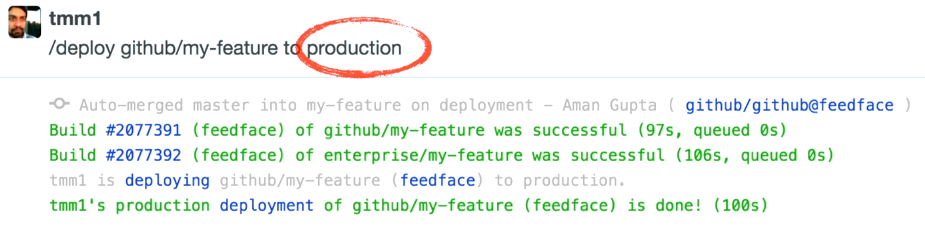
\includegraphics[scale=0.5]{images/SlackDeploy.png}
            \end{center}
            \caption{Exemple d'une commande de déploiement dans Slack}
            \label{SlackDeploy}
          \end{figure}

          \paragraph{La queue de déploiement} Pendant les heures de pointe de travail, plusieurs développeurs essaient souvent de déployer simultanément leurs changements dans le même environnement. Pour éviter toute confusion et donner une chance à tous de déployer, nous ajoutons à Hubot une file d'attente de déploiement. Les développeurs désirant déployer doivent ainsi s'enregister auprès d'Hubot et attendre leur tour. Cette nouvelle fonctionnalité s'appuie sur trois commandes.
          La première des trois - « /hubot queue » - permet de connaître l'état en cours de la file de déploiement de l'environnement passée en paramètre. Hubot nous renverra la liste des développeurs en attente de déploiement.
          La seconde commande - « /hubot queueme » - permet aux développeurs de s'enregistrer dans la queue de déploiement de l'environnement passée en paramètre.
          La troisième commande - « /hubot unqueueme » - permet aux développeurs présents dans la file de l'environnement passée en paramètre de s'en retirer.

          \paragraph{Le verrou de déploiement} Toujours dans une optique de déploiement simultané sur un même environnement nous devons implémenter une fonctionnalité de verrouillage sur la branche déployée afin que l'intégralité des tests soient effectués avant le déploiement d'une nouvelle version. Pour cela nous ajoutons à notre script de déploiement Hubot une instruction chargée de gérer le verrou des environnements.

          \paragraph{La maintenance applicative} La plupart des équipes de développement dispose d'un outil de suivi de bugs afin de tracer et corriger les disfonctionnements de leurs applications liées aux erreurs de développement. Qu'elle fonctionne sur le principe de carte (Jira) ou d'issue (Github), notre chatroom doit être en capacité de retranscrire le bug dans le flux de conversation du projet. Le bug est ainsi directement pris en compte par l'équipe de développement et corrigé rapidemment. Les développeurs doivent aussi être en mesure de clore les cartes ou issues une fois celles-ci traitées. Pour cela nous allons ajouter un troisième paramètre à notre commande de déploiement spécifiant l'identifiant du disfonctionnement retourné par l'outil de suivi de bugs.

          \paragraph{La sécurité} Un des points importants au sein des services informatiques est la sécurité des serveurs. Avec un script Hubot, nous pouvons gérer l'accés aux différents serveurs en fonction des collaborateurs selon un principe d'autorisation; seules les personnes autorisées peuvent effectuer des actions sur les environnements. De plus, notre plate-forme d'Intégration Continue garantit la confidentialité des chaînes de connexion et des mots de passe des serveurs. L'intégralité des données de connexion aux environnements et l'accès à ces derniers étant gérés par Hubot, les risques de perte ou de fuite de ces informations critiques sont ainsi minimisés.

      \subsection{Architecture et fonctionnement de la PIC}
      Dans sa version finale, notre plate-forme d'Intégration Continue est composée d'un serveur permanent « maître » dans le Cloud Amazon Web Services - hébergeant Mattermost (outil de communication asynchrone) le point d'entrée de notre PIC, Hubot (outil d'exécution de scripts) notre robot intelligent et Ansible notre outil de provisionning d'instance - et d'instances éphémères « esclaves », elles aussi dans le Cloud AWS, qui accueillent notre serveur d'Intégration Continue GoCD.\\

      Du point de vue du fonctionnement, nos équipes de travail intéragissent indirectement avec le serveur d'Intégration par le biais de lignes de commande via les chatrooms présentent au sein de la plate-forme de communication et Hubot (Voir Figure \ref{PICv3}).\\

      Comme dans notre version précédente, l'intégralité des déploiements, « maître » comme « esclave », est automatisé et géré par Ansible.

      \begin{figure}
        \begin{center}
          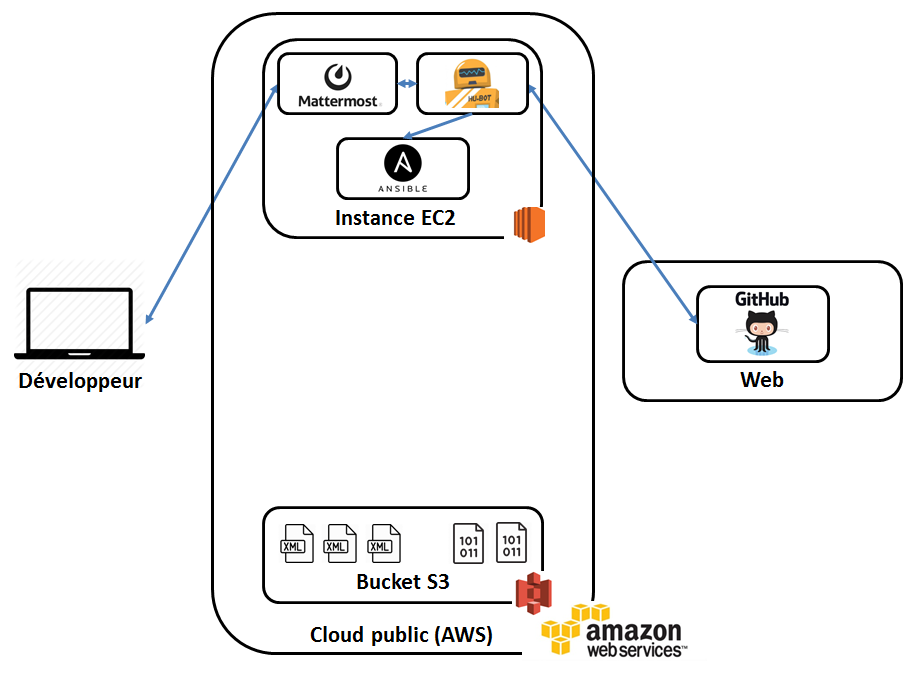
\includegraphics[scale=0.5]{images/PICv3.png}
        \end{center}
        \caption{Schéma de la troisième version de notre PIC - Cloud II}
        \label{PICv3}
      \end{figure}

      \section{Aller plus loin}
      Avant de poursuivre avec l'ultime chapitre de ce mémoire qui a pour vocation de proposer des axes d'améliorations et de nouvelles fonctionnalités à notre solution, nous allons faire un petit récapitulatif des outils, des caractéristiques et des fonctionnalités de notre plate-forme d'Intégration Continue. Pour les outils, nous avons utilisé:\\

      \begin{itemize}
        \item un serveur d'Intégration Continue (GoCD),
        \item un référentiel de code source (Git/Github),
        \item un fournisseur de Cloud (Amazon Web Service),
        \item un provisionneur d'instances (Ansible),
        \item un exécuteur de scripts (Hubot),
        \item une plate-forme de communication asynchrone (Mattermost).\\
      \end{itemize}

      Du côté des caractéristiques notre solution est:\\

      \begin{itemize}
        \item multi-plateformes (Windows et Linux),
        \item multi-langages (.NET, JAVA/J2EE, Javascript, ...),
        \item multi-référentiels de code source (Git, TFS, SVN, ...),
        \item open source,
        \item automatisée,
        \item « First Class »,
        \item « Infrasctucture As Code »,
        \item à la demande.
      \end{itemize}

      Et a pour fonctionnalités :\\

      \begin{itemize}
        \item l'intégration,
        \item l'exécution des analyses statiques du code,
        \item la build,
        \item l'exécution des tests,
        \item la création de rapports,
        \item la création de documentation,
        \item le déploiement,
        \item la maintenance,
        \item la sécurité.\\
      \end{itemize}

      Nous constatons que notre solution répond à l'intégralité des critères de l'Intégration Continue vus en première partie de ce mémoire (Voir le Chapitre \ref{ContinousIntegration}). Mais de nombreuses autres problématiques liées aux cycles de vie des applications et aux développements en eux-mêmes peuvent être greffées à notre plate-forme. Nous allons en voir quelques unes et essayer d'offrir des pistes de reflexion quant à leur intégration.

      \subsection{Les analyses, le monitoring et les alertes}
      Il peut s'avérer très intéressant pour les équipes, de travailler avec des rapports d'analyses contrôlant les performances, les charges, les disponibilités, l'utilisation des fonctionnalités, etc de leurs applications. Les applications de monitoring perforent le marché des solutions informatiques et sont de plus en plus sollicitées par les organisations. Il peut s'avérer utile d'intégrer des commandes à notre plate-forme d'Intégration Continue permettant d'avoir une représentation graphique des diverses analyses dans nos chatrooms. Au vue des nombreux acteurs de monitoring et des solutions développées en interne il est difficile de conjecturer sur une solution générique, vous devrez sans doute développer votre propre script Hubot.\\

      Mais plus que monitorer pour monitorer, les équipes de travail désirent surtout recevoir des alertes lorsque les seuils fixés sont atteints et que le fonctionnement de l'application devient critique. Votre script devra être capable d'écouter - c'est la solution à privilégier - ou interroger à des intervalles de temps réguliers vos outils de monitoring. Les développeurs seront ainsi rapidement et efficacement prévenus des dysfonctionnements de l'application.

      \subsection{La remontée automatique des dysfonctionnements lié au code}
      Les dysfonctionnements d'une application peuvent être de natures diverses; nous avons les bugs techniques, les bugs liés au code, les bugs d'utilisation... Cependant ils ont une chose en commun, ils doivent être résolus rapidemment sous peine d'endommager le fonctionnement de l'application. Principalement, les bugs impactants les developpeurs, sont ceux liés au code - qu'ils soient fonctionnels, de conception ou liés au langage. Si l'application dispose d'une remontée d'erreur efficace, la source du dysfonctionnement (trace d'appel ou « \gls{stack trace} ») est archivée dans un fichier de logs et permet ainsi aux équipes d'en comprendre la provenance et de la corriger en un rien de temps. Nous constatons malheureusement que le temps de correction d'un bug est anormalement élevé, ce qui favorise sa reproduction. En étudiant son cycle de vie (celui de la correction du bug) nous remarquons que ce temps n'est pas dû à la correction du bug en lui-même mais en sa prise de connaissance de la part des développeurs. Il peut alors être très utile de disposer d'un service de remontée automatique pour les dysfonctionnements liés au code, directement dans la chatroom de l'équipe. La remontée pourrait se faire sous forme d'alerte, indiquant la stack trace et le nom du dernier développeur ayant modifié la portion de code impactée.\\

      Au niveau de la mise en place nous partons sur l'idée d'un \gls{ETL}\footnote{Extract-Transform-Load: technologie informatique intergicielle (middleware) permettant d'effectuer des synchronisations massives d'information d'une source de données vers une autre.} destiné aux logs tel que Logstash (open source) qui écouterait les fichiers de logs et transférerait les nouveaux logs d'erreurs à Hubot. Ce dernier n'aurait plus qu'à alerter Mattermost.

      \subsection{Un dépôt de plate-forme d'Intégration Continue}
      Afin de poursuivre dans l'optique de l'open source il pourrait être intéressant de mettre à la disposition des développeurs un dépôt permettant d'archiver et de partager les diverses configurations de leurs Plate-formes d'Intégration Continue. Elles seraient classées par système d'exploitation et par langage de programmation. La mise en place et la configuration du serveur et des pipelines de déploiement seraient ainsi d'une simplicité élémentaire et permettraient à tous de bénéficier d'une Intégration Continue optimale.


  \listoffigures                  % Liste les figures
  \bibliographystyle{alpha}       % les trois premières lettres du nom de l'auteur accolées aux deux derniers chiffres de l'année de parution
  \bibliography{MemoireM2}        % mon fichier de base de données s'appelle MemoireM2.bib
  \appendix
  \chapter{Cloud Computing} \label{CloudComputingAnnexe}

  \section{Définition}
  Il existe autant de réponse à « Qu’est-ce que le Cloud Comptine ? » que de distribution linux. J’ai pour ma part décider de baser mon analyse sur la définition fournit par NIST (National Institut of Standards and Technology):\\

  \begin{quotation}
    \emph{« Cloud Computing is a model for enabling ubiquitous, convenient,on-demand network access to a shared pool of configurable Computing resources (e.g., networks, servers, storage, applications, and services) that can be rapidly provisioned and released with minimal management effort or service provider interaction. This Cloud model is composed of five essential characteristics, three service models, and four deployment models. »}
  \end{quotation}

  \begin{quotation}
    \emph{« Le Cloud Computing est un modèle qui permet un accès omniprésent, pratique et à la demande à un réseau partagé et à un ensemble de ressources informatiques configurables (comme par exemple : des réseaux, des serveurs, du stockage, des applications et des services) qui peuvent être provisionnées et libérées avec un minimum d’administration. »}\\
  \end{quotation}

  Pour simplifier, le Cloud Computing est la dématérialisation de l’informatique. C’est le fait de déporter toutes les opérations normalement effectuées sur nos ordinateurs sur des machines distantes, autrement dit sur internet. L’ensemble de ses serveurs constitue le Cloud (Voir Figure \ref{Cloud Computing}).

  \begin{figure}
    \begin{center}
      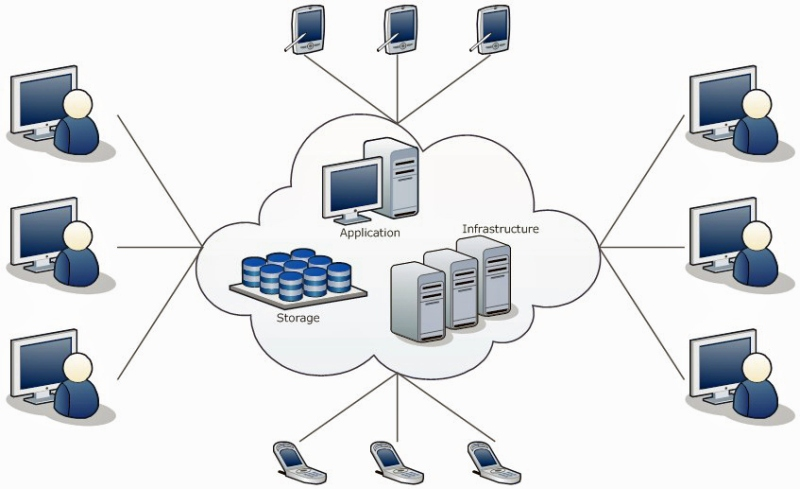
\includegraphics[scale=0.3]{images/CloudComputing.png}
    \end{center}
    \caption{Schématisation du Cloud Computing}
    \label{Cloud Computing}
  \end{figure}

  \subsection{Un service à la demande et une flexibilité des ressources.}
  Avec les applications Cloud, nous adaptons le flux de données à l'évolution de nos besoins: nous ne payons que ce que nous consommons. Et nous n'avons plus à nous soucier du manque de capacité.

  \subsection{Accès universel par le réseau}
  Le terme de nuage représente bien le concept. Imaginons que nos ordinateurs nous suivent partout, que nous puissions y accéder n’importe où, n’importe quand depuis n’importe quel terminal (ATAWAD - « AnyTime, AnyWhere, AnyDevice »). Imaginons un accès universel aux ressources stockées sur nos ordinateurs.

  \subsection{Une mise en commun des ressources}
  L'application de correctifs, la mise à niveau et le tests d'application peuvent occuper nos équipes informatiques plusieurs jours par mois. Grâce aux applications Cloud, cette problématique disparaît.\\

  Cependant ce n’est pas si simple que cela. Il existe trois types de Cloud: le Cloud public (loué par des prestataires), le Cloud privé (créer et gérer par notre entreprise) et le Cloud hybride (un mélange des deux précédents).

  \section{Le Cloud public}
  Le Cloud public appartient à des prestataires de service qui louent l’utilisation de leurs serveurs en facturant leur utilisation à la demande. Nous payons le flux de données échangé. Il dispose principalement de quatre modèles qui correspondent à des besoins bien distincts: le IAAS, le PASS, le SAAS et le STAAT.

    \subsection{Le Cloud IAAS ou Infrastructure As A Service (infrastructure en tant que service)}
    Le IAAS correspond à une infrastructure informatique (serveurs, réseaux, stockage) hébergée chez le prestataire de service. Nous n’avons pas besoin d’acheter le matériel nécessaire à notre infrastructure, nous nous contentons de la louer mais la gérons comme bon nous semble. Nous déployons les serveurs que nous souhaitons utiliser et nous gérons l’ensemble des OS installés sur ces derniers. IAAS est utile si l’on désire créer ses propres plateformes pour ensuite y héberger nos applications comme sur des serveurs locaux.

    \subsection{Le Cloud PAAS ou Plateform As A Service (plateforme en tant que service)}
    Le PAAS constitue l’utilisation par le biais d’internet de plateformes sur lesquelles nous pouvons déployer nos propres applications. C’est le niveau d’exécution des logiciels. Nous louons une plateforme, c’est à dire une machine avec un OS, le tout prêt à l’emploi.

    \subsection{Le Cloud SAAS ou Software As A Service (logiciel en tant que service)}
    Il s’agit d’utiliser des logiciels directement sur le Cloud, la plupart du temps via un navigateur web. Nous n’avons pas d’achat de licence, pas d’installation sur nos propres terminaux, pas d’entretien. Le logiciel « tourne » sur des serveurs dans des datacenters (Voir Figure \ref{Google Cloud}).

    \begin{figure}
      \begin{center}
        
\includegraphics[scale=1]{images/googleDrive.png}
      \end{center}
      \caption{Exemple: la suite bureautique proposée par Google}
      \label{Google Cloud}
    \end{figure}

    \subsection{Le STAAT ou Storage As A Service (stockage en tant que service)}
    Le STAAT permet simplement des stocker nos données.

  \section{Le Cloud privé}
  Le Cloud privé est un Cloud propre à notre entreprise. A l’aide d’outils de virtualisation, il est possible de transformer les serveurs existants au sein de l’entreprise en serveur Cloud. Cela créé un réseau puissant, disponible - comme le Cloud public - à tout moment et à tout endroit mais géré entièrement par notre entreprise.

  \section{Las avantages du Cloud Computing}
  Les avantages du Cloud Computing sont nombreux. Si l’accessibilité est l’avantage le plus visible, il faut remarquer que l’utilisation du Cloud Computing permet à l’entreprise d’avoir une grande agilité, allant du démarrage rapide de son activité à un déploiement tout aussi rapide de nouvelles applications et donc un gain de temps et d’argent pour l’entreprise.\\

  De plus avec l’utilisation d’un Cloud public l’entreprise n’a plus d’investissement lourd en capital informatique, plus de dépendance en perte de temps et en entretient des infrastructures. Gains de places et de performances sont au rendez-vous.\\

  Cependant il faut soulever un petit bémol. En effet la contrepartie de tous cela est une dépendance totale envers internet et les prestataires de service. Ainsi qu’un coût croissant à mesure que les besoins de l’entreprises grandissent.

  \section{Quel Cloud choisir?}
  Si nous disposons déjà de serveurs et que nos besoins sont constants nous opterons pour le Cloud privé. Nous virtualiserons notre infrastructure et profiter de notre propre Cloud. Nos investissements sont ainsi préservés et nous gagnerions en productivité.\\

  En revanche, si nous ne disposons pas de serveurs ou que nous commençons tout juste notre activité et que nous ne souhaitons pas investir dans un parc informatique de serveur complet nous opterons pour un Cloud public. Economie et flexibilité sont au rendez-vous avec les services à la demande.\\

  Enfin si nous possédons des serveurs mais que notre activité fluctue beaucoup, nous demandant parfois des capacités plus fortes, nous opterons pour le Cloud hybride. Nous conserverons ainsi notre autonomie avec notre Cloud privé et étendrons notre capacité ponctuellement avec le Cloud public.\\

  Pour conclure, si le Cloud Computing offre une grande disponibilité et une adaptabilité exemplaire, qui en font un service formidable, il n’en reste pas moins dépendant d’internet et les risques en matières de sécurité sont encore mal évalués.
\label{CloudComputing}
\end{document}
